\section{The effect of ageing on turquoise killifish antibody repertoires}
\label{sec:igseq_ageing}

\newabbreviation{GLM}{GLM}{Generalised linear model}

The pilot study into the antibody repertoires of mature adult turquoise killifish (\Cref{sec:igseq_pilot}) demonstrated that... % TODO: Briefly summarise importance of pilot results
However, ... % TODO: Segue into testing across age

In order to investigate the effects of ageing on the killifish antibody repertoire, In order to investigate the effect of ageing on these processes, each of the 32 fish described in  \Cref{tab:igseq-cohorts-summary,tab:igseq-cohorts-fish} % TODO: Figure of age groups? Describe better?
underwent two independent library preparations as described in \Cref{sec:methods_molec_igseq} and \Cref{sec:igseq_protocol_library}, % TODO: Table of cycle numbers etc.
for a total of 64 pooled libraries; these were then sequenced together in two MiSeq runs, yielding a total of \embed{_Figures/txt/ageing-reads-raw-total.txt} million read pairs (\embed{_Figures/txt/ageing-reads-raw-replicate-min.txt} to \embed{_Figures/txt/ageing-reads-raw-replicate-max.txt} million pairs per replicate, \embed{_Figures/txt/ageing-reads-raw-individual-min.txt} to \embed{_Figures/txt/ageing-reads-raw-individual-max.txt} million pairs per individual), and the resulting reads underwent pre-processing, filtering and clonotyping as described in \Cref{sec:igseq_protocol_preprocess,sec:igseq_pilot_composition,sec:igseq_pilot_clones}.

\Cref{fig:igseq-ageing-read-survival-all} shows the absolute and relative read survival for each of the sixty-four sequencing libraries throughout this process. As with the pilot dataset, the replicates show relatively consistent behaviour up to and including VDJ assignment and Change-O database construction, with \embed{_Figures/txt/ageing-read-survival-init-min.txt}\,\% to \embed{_Figures/txt/ageing-read-survival-init-max.txt}\,\% of reads surviving up to this stage in the pipeline. However, a somewhat larger number of sequences (\embed{_Figures/txt/ageing-read-survival-rel-loss-total.txt}\,\%, up to \embed{_Figures/txt/ageing-read-survival-rel-loss-max.txt}\,\% per replicate) are lost during V-score filtering compared to the pilot dataset (\embed{_Figures/txt/pilot-read-survival-rel-loss-total.txt}\,\%, up to \embed{_Figures/txt/pilot-read-survival-rel-loss-max.txt}\,\% per replicate). This inconsistency is due to a greater preponderance in the ageing dataset of malformed, J-identity-lacking sequences, which in this case actually make up an absolute majority of unique sequences in the \program{pRESTO}-processed dataset (\Cref{fig:igseq-ageing-functional-prop-pre}). After filtering on V-score, however, the functional composition of the ageing dataset is similar to that of the pilot data (\Cref{fig:igseq-ageing-functional-prop-post,fig:igseq-pilot-functional-prop-b}).

\begin{figure}
\centering
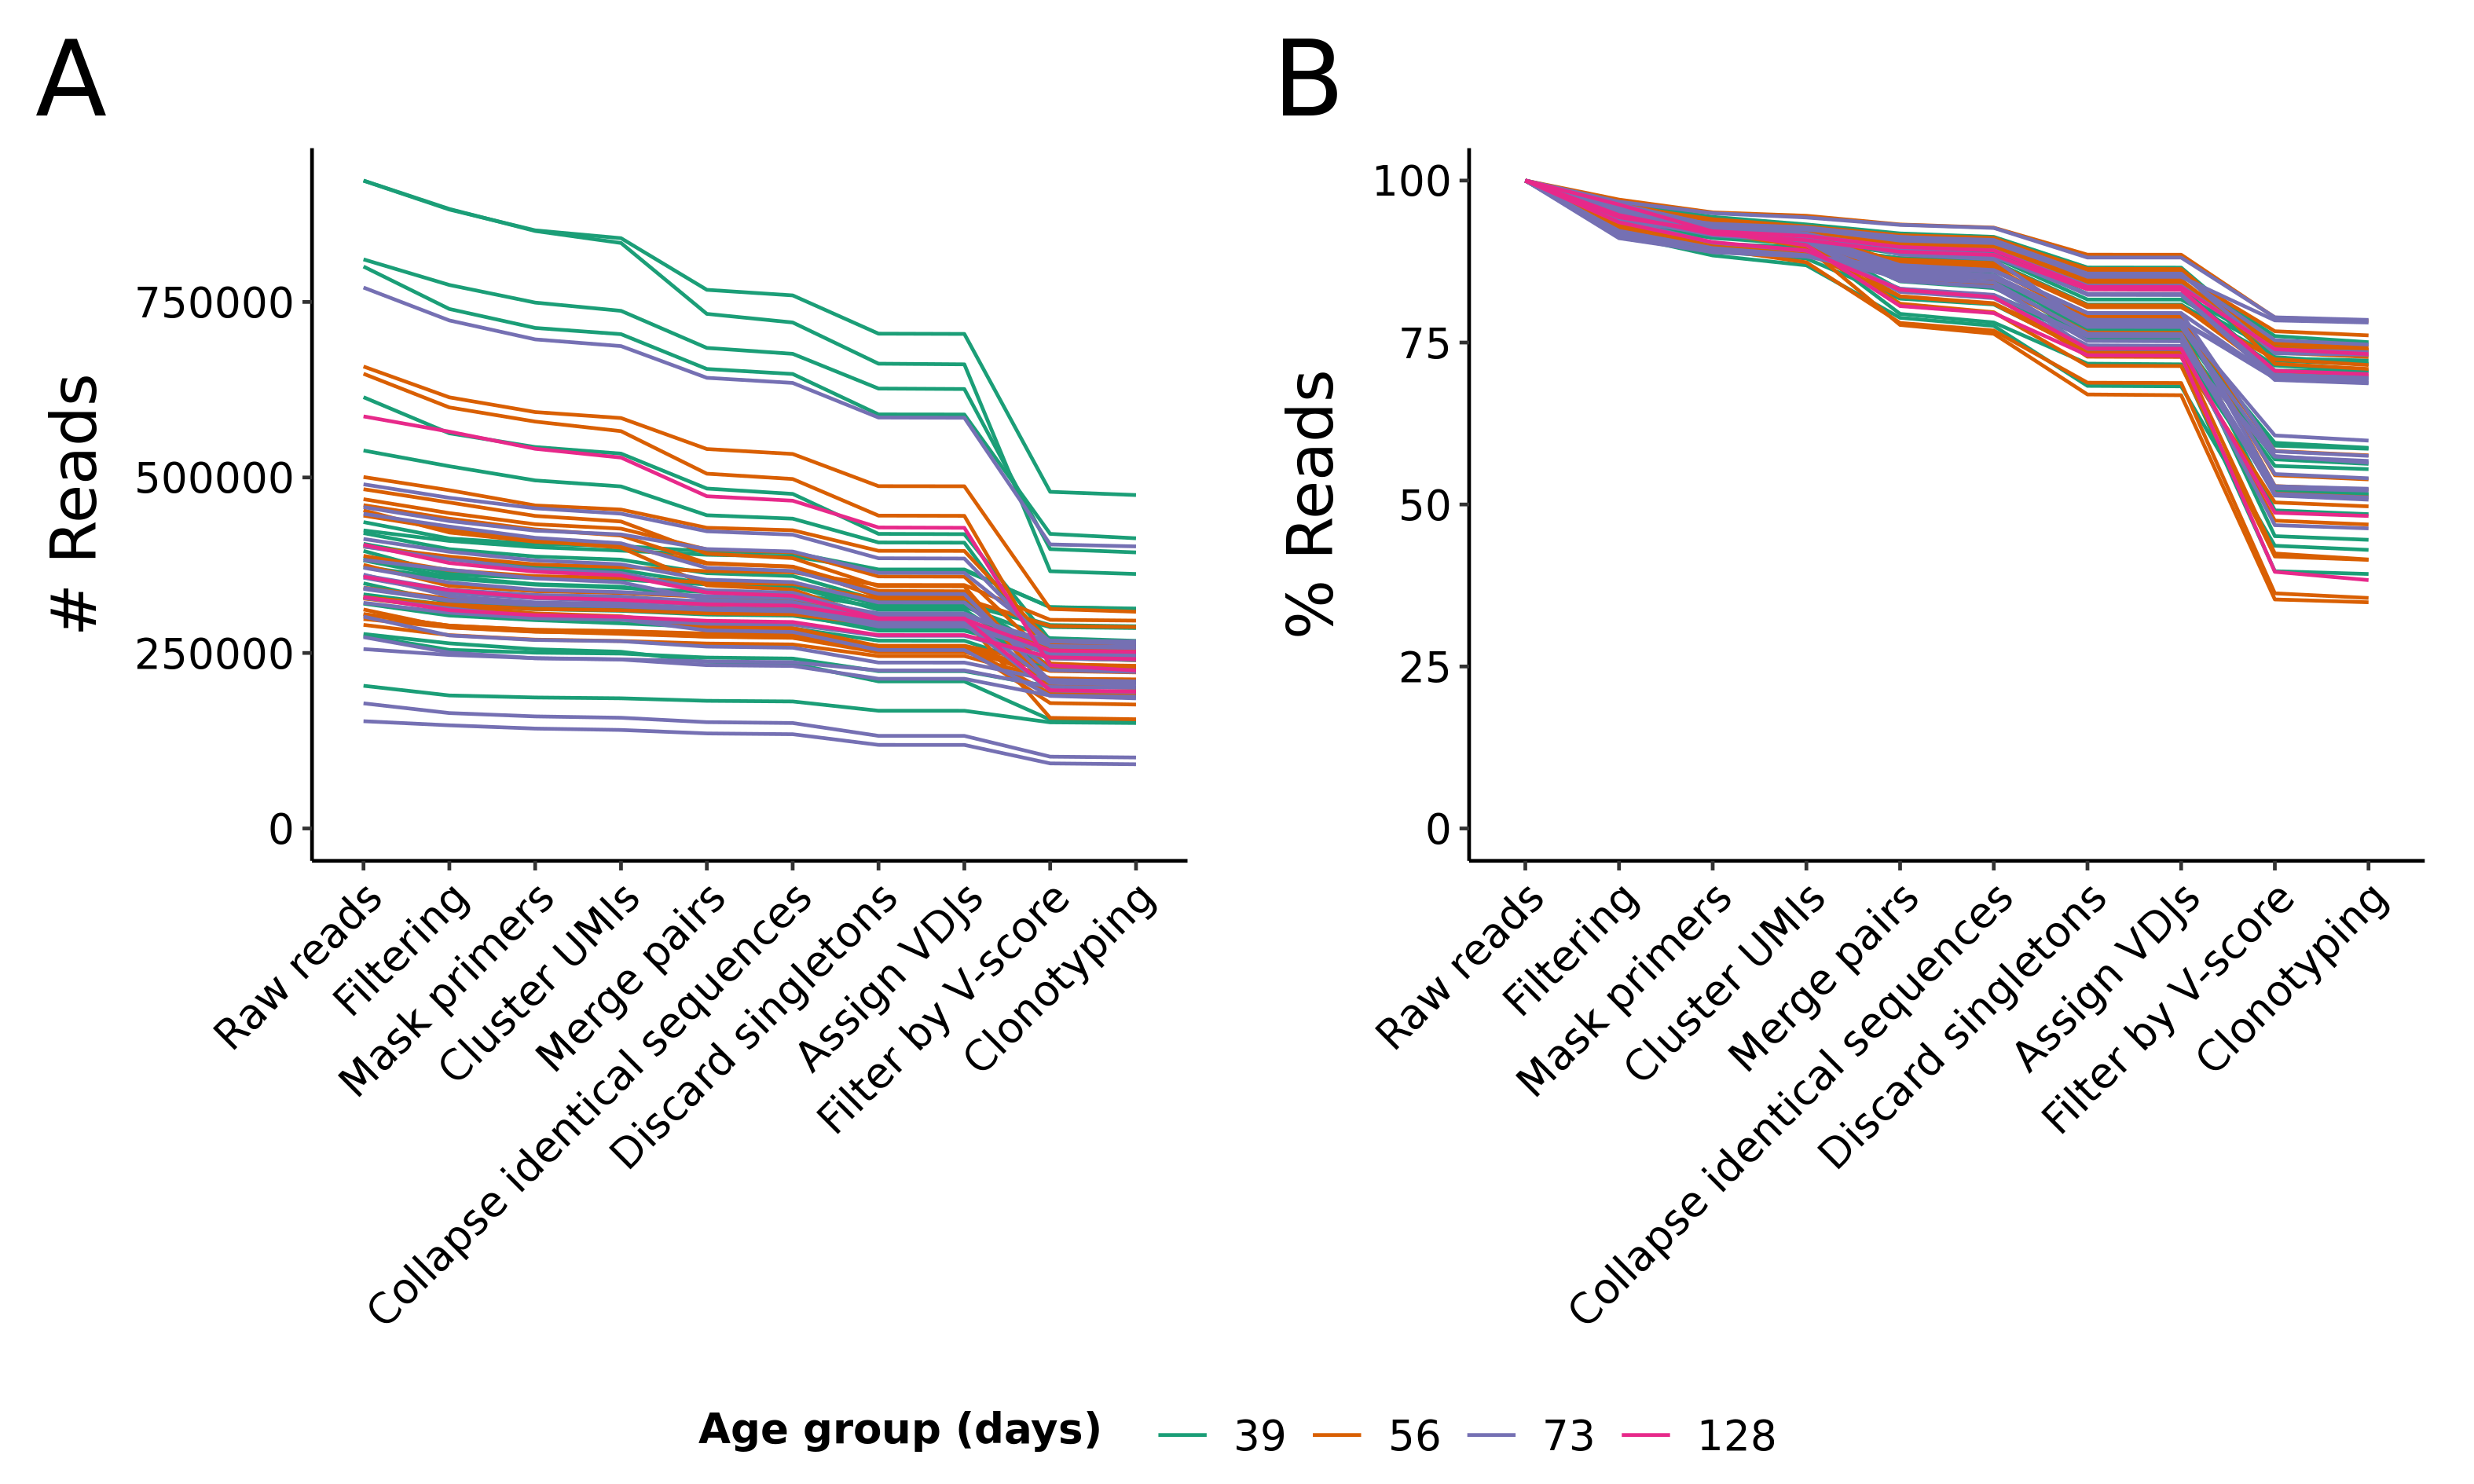
\includegraphics[width = 0.9\textwidth]{_Figures/png/ageing-read-survival-all.png}
\begin{subfigure}{0em}
\phantomsubcaption{}
\label{fig:igseq-ageing-read-survival-all-abs}
\end{subfigure}
\begin{subfigure}{0em}
\phantomsubcaption{}
\label{fig:igseq-ageing-read-survival-all-rel}
\end{subfigure}
\caption[Read survival during pre-processing of \igseq ageing dataset]{\textbf{Read survival during pre-processing of \igseq pilot dataset:} Line graphs of absolute (A) and relative (B) read survival during pre-processing of the \igseq ageing dataset, up to and including clonotyping.}
\label{fig:igseq-ageing-read-survival-all}
\end{figure}

\begin{figure}
\centering
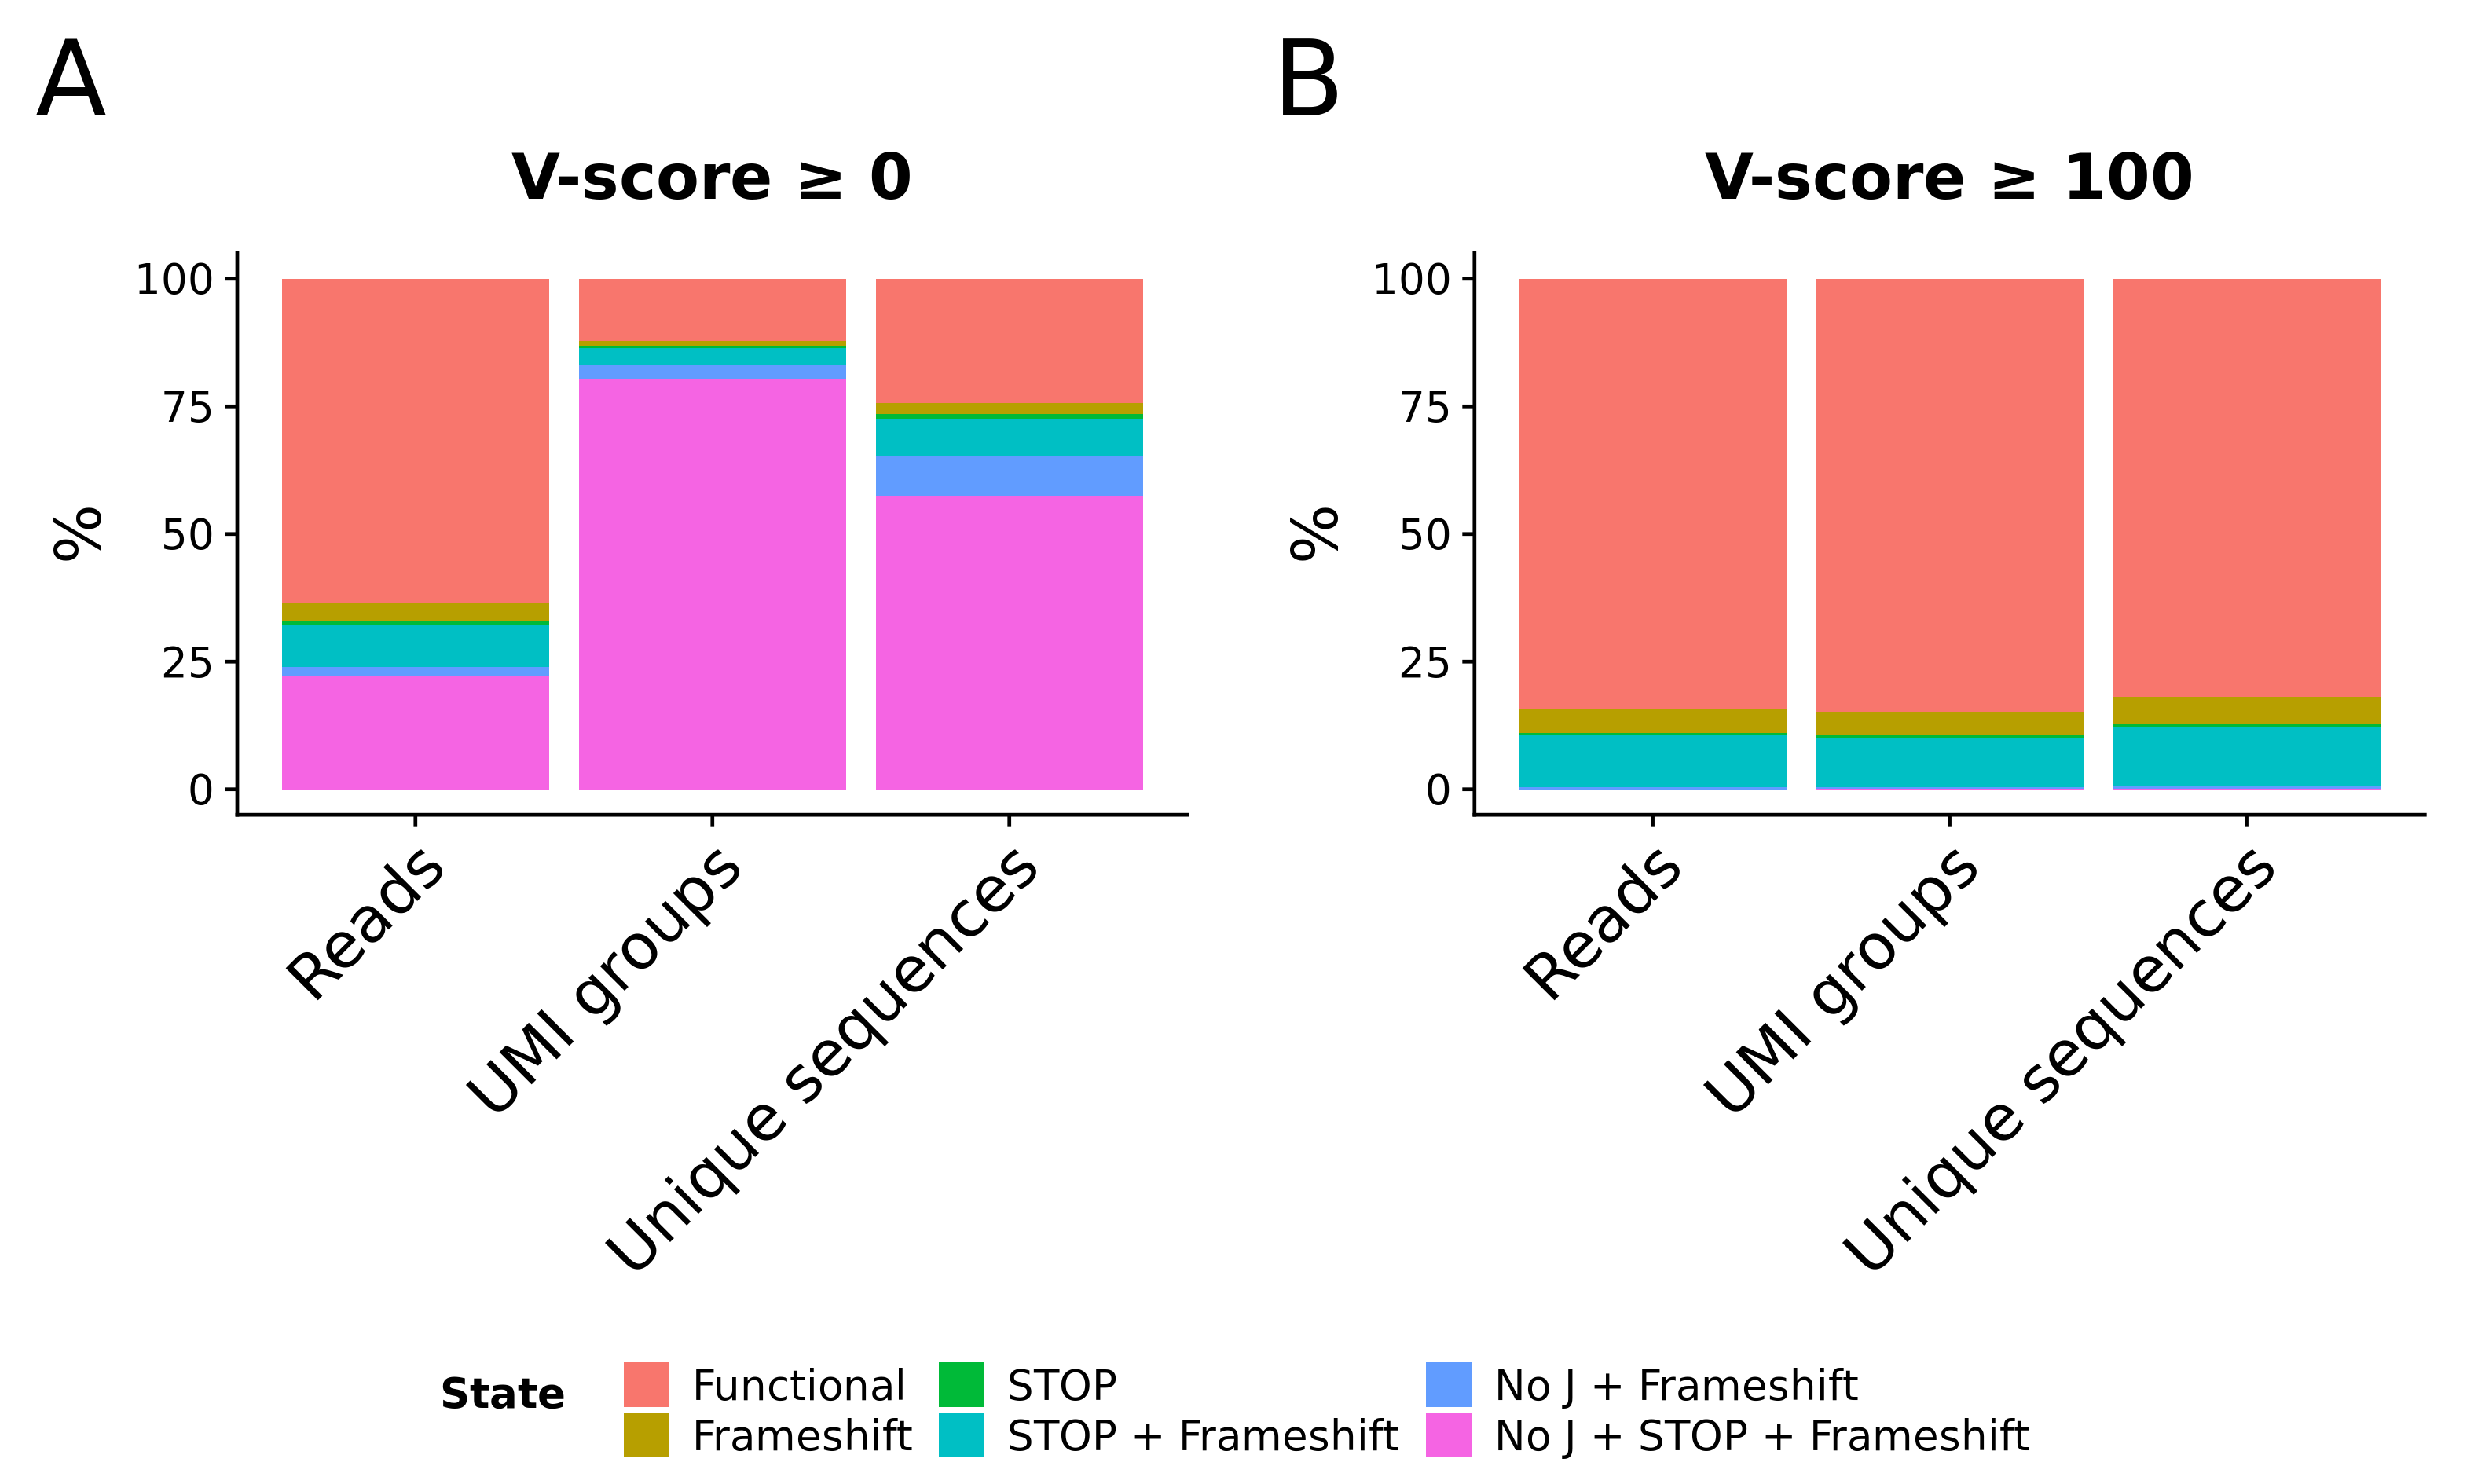
\includegraphics[width = 0.9\textwidth]{_Figures/png/ageing-functional-prop}
\begin{subfigure}{0em}
\phantomsubcaption{}
\label{fig:igseq-ageing-functional-prop-pre}
\end{subfigure}
\begin{subfigure}{0em}
\phantomsubcaption{}
\label{fig:igseq-ageing-functional-prop-post}
\end{subfigure}
\caption[Functional composition and V-score filtering of \igseq ageing dataset]{\textbf{Functional composition and V-score filtering of \igseq ageing dataset:} Proportion of input reads, UMI groups and unique sequences in the \igseq ageing dataset belonging to different (non)functional categories, before (A) and after (B) filtering on V-alignment score.}

\label{fig:igseq-ageing-functional-prop}
\end{figure}

Following V-score filtering, \embed{_Figures/txt/ageing-nseq-assigned-clones.txt}\,\% of remaining unique sequences in the ageing dataset were successfully assigned clonal identities. The number of clones inferred per individual ranged from \embed{_Figures/txt/ageing-nclones-individual-min.txt} to \embed{_Figures/txt/ageing-nclones-individual-max.txt}, with a median of \embed{_Figures/txt/ageing-nclones-individual-med.txt}; there is a non-significant (Kruskal-Wallis analysis of variance, $p=\embed{_Figures/txt/ageing-nclones-kruskal-p.txt}$) decline in number of clones per individual with age (\Cref{fig:igseq-ageing-nclones}). These clonal counts are much lower than the median of \embed{_Figures/txt/pilot-nclones-individual-med.txt} clones per individual for the pilot study, reflecting the lower number of reads per individual available in this dataset; for comparison, for the four individuals included in the pilot study, the number of identified clones in the ageing dataset ranges from \embed{_Figures/txt/ageing-nclones-individual-min-pilot.txt} to \embed{_Figures/txt/ageing-nclones-individual-max-pilot.txt}. Concordantly, the distribution of clone sizes detected in the ageing dataset is even more skewed towards small clones than in the pilot dataset: \embed{_Figures/txt/ageing-nclones-pc-1count.txt}\,\% of clones are observed as just a single unique sequence across all replicates, while \embed{_Figures/txt/ageing-nclones-pc-small.txt}\,\% contain fewer than five unique sequences (\Cref{fig:igseq-ageing-clone-sizes-sizes}). As in the pilot dataset, larger clones were much more likely to be observed across both replicates for a given individual  (\Cref{fig:igseq-ageing-clone-sizes-reps}).

\begin{figure}
\centering
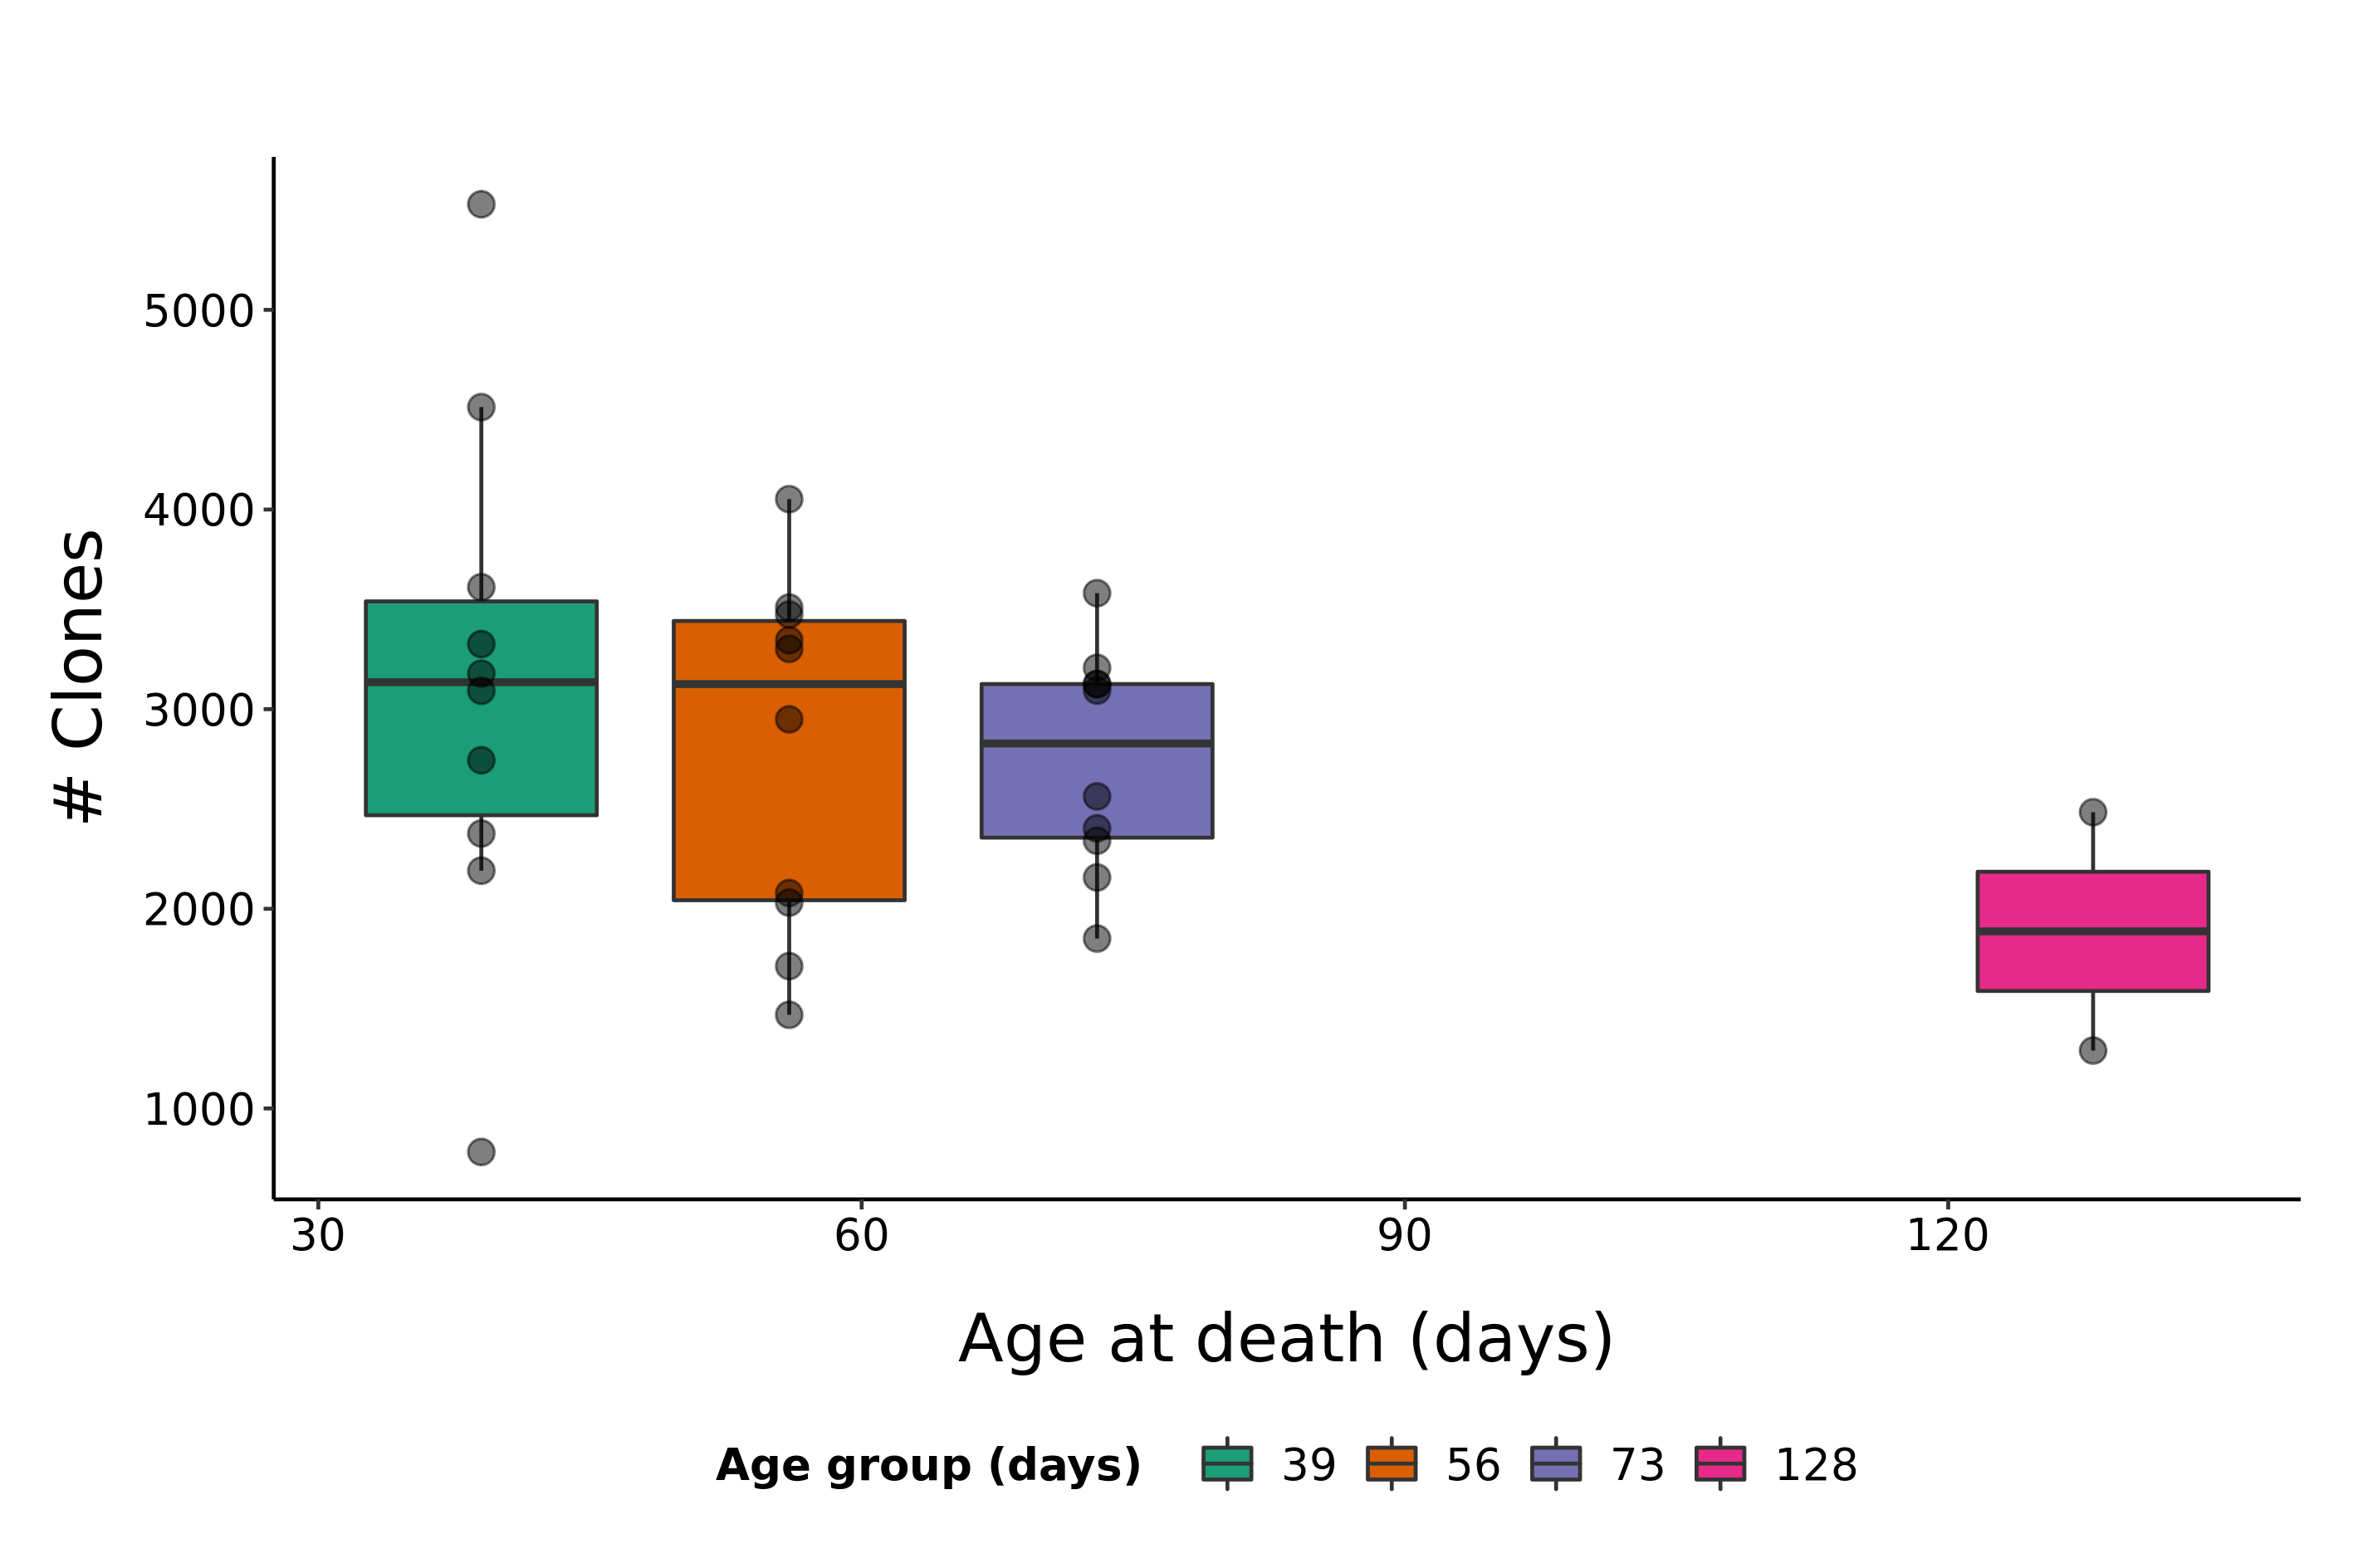
\includegraphics[width = 0.8\textwidth]{/home/will/Documents/thesis/_Figures/png/ageing-nclones.png}
\caption[Number of clones in the \igseq ageing dataset]{\textbf{Number of clones in the \igseq ageing dataset:} Boxplots of clonal counts for each individual in the \igseq ageing dataset, grouped by age at death. The apparent decline in clonal count with age is not significant (Kruskal-Wallis analysis of variance, $p=\embed{_Figures/txt/ageing-nclones-kruskal-p.txt}$).}
\label{fig:igseq-ageing-nclones}
\end{figure}

\begin{figure}
\centering
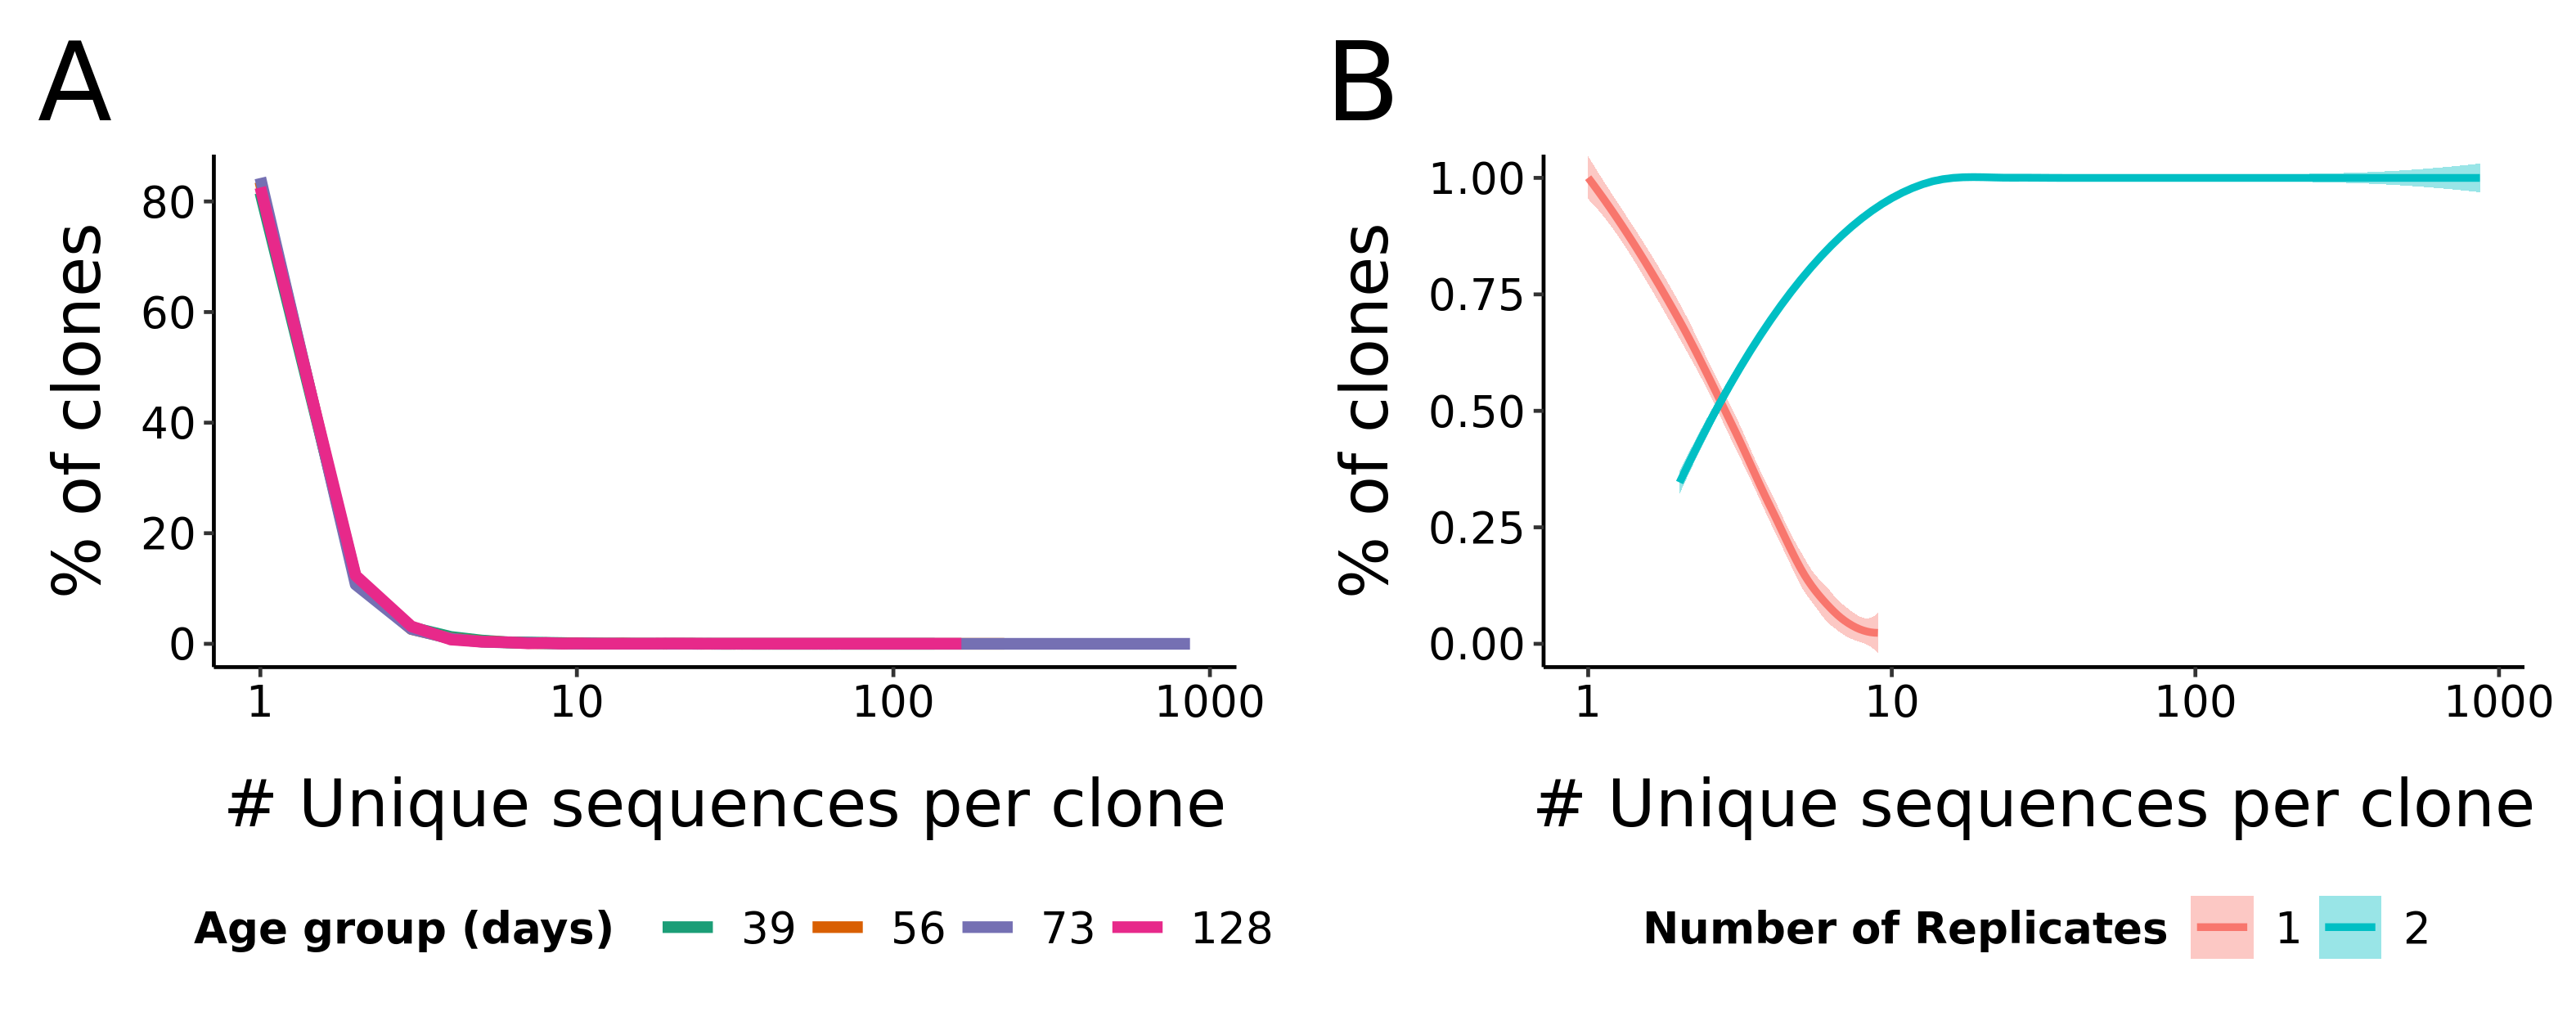
\includegraphics[width = 0.9\textwidth]{_Figures/png/ageing-clone-sizes}
\begin{subfigure}{0em}
\phantomsubcaption{}
\label{fig:igseq-ageing-clone-sizes-sizes}
\end{subfigure}
\begin{subfigure}{0em}
\phantomsubcaption{}
\label{fig:igseq-ageing-clone-sizes-reps}
\end{subfigure}
\caption[Clone size and cross-replicate reproducibility in the \igseq ageing dataset]{\textbf{Clone size and cross-replicate reproducibility in the \igseq ageing dataset:}(A) Proportion of clones of different sizes for each individual in the ageing dataset, measured in unique sequences per clone. (B) LOESS-smoothed curves showing proportion of clones of each size found across one or both replicates of the appropriate individual.}
% TODO: Add suitable overall figure title
\label{fig:igseq-ageing-clone-sizes}
\end{figure} % TODO: Citation for LOESS smoothing

\begin{figure}
\centering
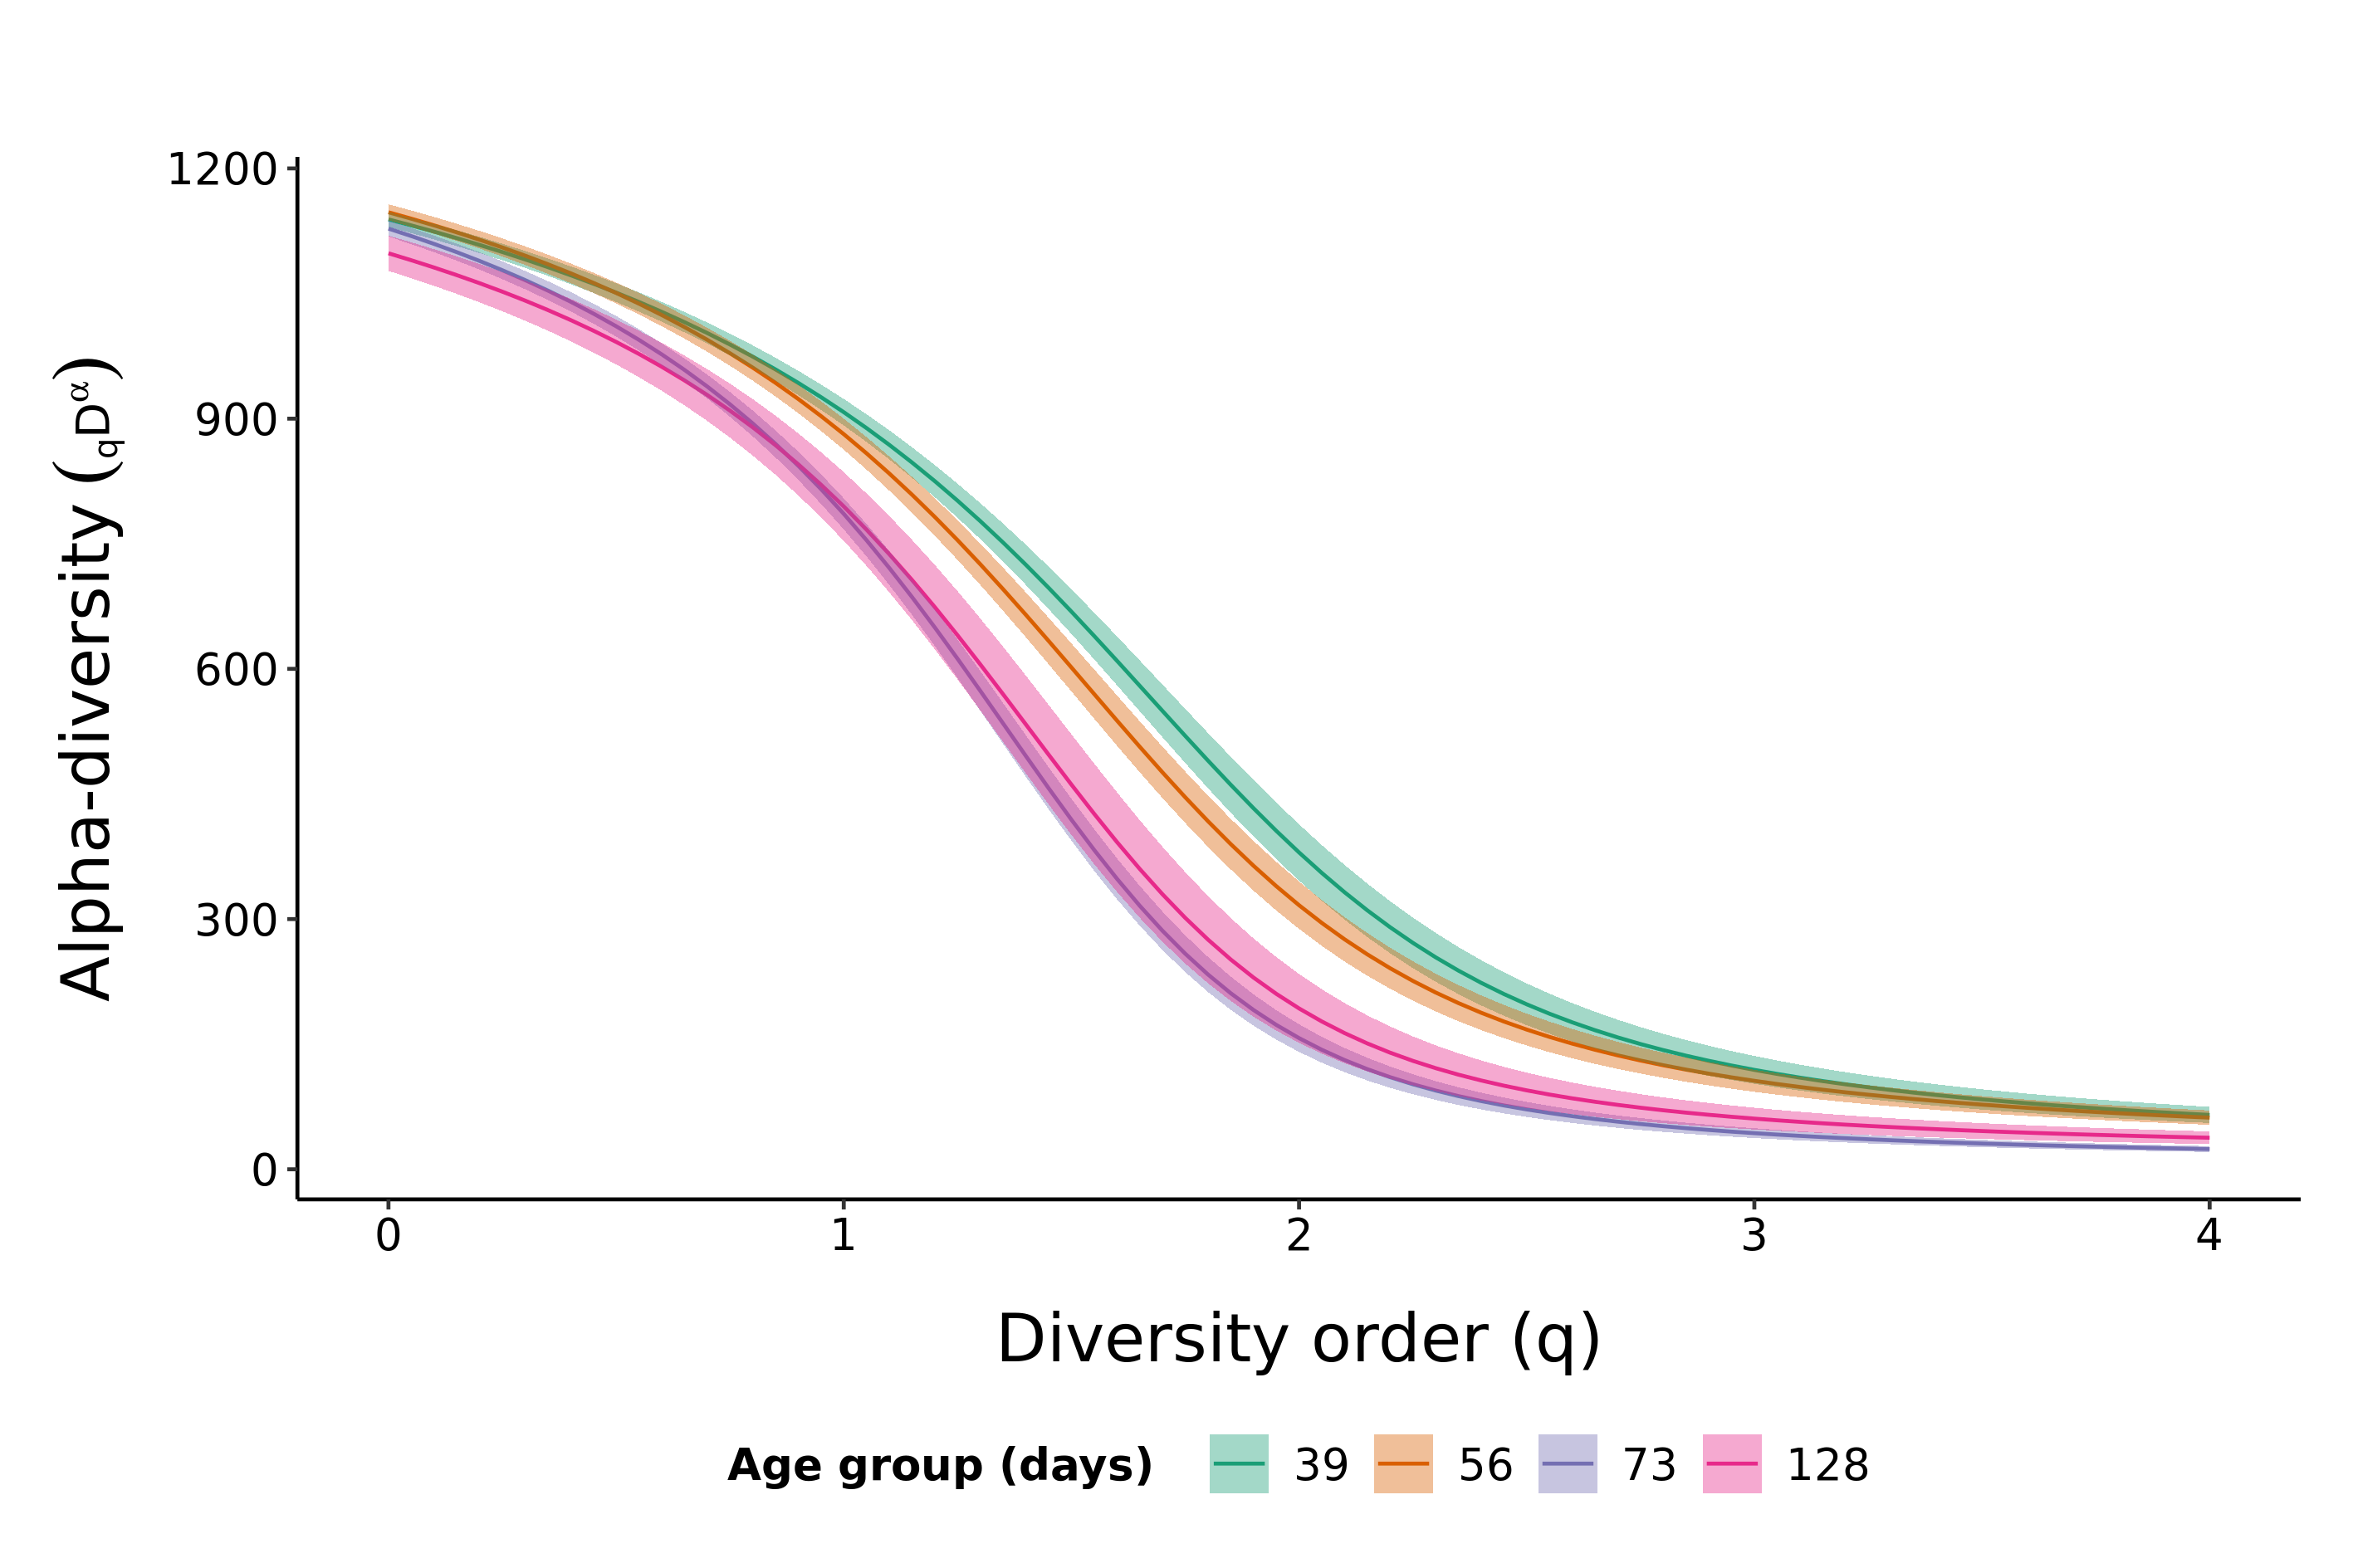
\includegraphics[width = 0.8\textwidth]{_Figures/png/ageing-clone-diversity-alpha}
\caption[Clonal alpha-diversity spectra for \igseq ageing dataset]{\textbf{Clonal alpha-diversity spectra for \igseq ageing dataset:} Bootstrapped alpha-diversity spectra of clone sizes for each age group in the \igseq ageing dataset, as measured by number of unique sequences per clone. Shaded regions in both subfigures represent 95\,\% confidence intervals, estimated using bootstrapping.}
\label{fig:igseq-ageing-clone-diversity-alpha}
\end{figure}

% TODO: Separate individual spectra in supplementary

In order to assess the effect of age on the clonal diversity of killifish antibody repertoires, the alpha-diversity spectrum of each age group (\Cref{app:diversity}) was computed as described in \Cref{sec:methods_comp_igdownstream_spectra,sec:igseq_pilot_clones}. The resulting spectra, shown in \Cref{fig:igseq-ageing-clone-diversity-alpha}, indicate that repertoire diversity declines monotonically between 5.5 and 10.5 weeks of age in the turquoise killifish, with the most rapid decline observed between 8 and 10.5 weeks: across the entire spectrum, the alpha-diversity of the 8-week group is the same as or lower than that of the 5.5 week group, the 10.5-week group is markedly less diverse than the 8-week group, and the 18-week and 10.5-week groups exhibit similar diversity. These observations suggest a model in which repertoire diversity begins declining before or at reproductive maturation (c. 5 weeks post-hatching), declines rapidly in later adulthood, and reaches a plateau of low diversity late in life; however, the smaller size of the 18-week-old group in comparison to the others means that the patterns observed in this group cannot be taken with confidence, and it is possible that a further decline after 10.5 weeks would be observed in a larger sample.

In order to test the significance of these differences in clonal diversity between age groups, the distributions of Hill diversity measurements at each of six diversity orders (0, 1, 1.5, 2, 3 and 4) were compared across age groups using two distinct methods. In the first, a generalised linear model (GLM) of diversity \textit{versus} age-at-death was fitted to each diversity order under a gamma distribution, and the resulting model was compared to a null (intercept-only) model to test for a significant ageing term; in the second, a non-parametric Kruskal-Wallis analysis of variance was used, again to test for a significant effect of age-at-death on the distribution of Hill diversities at a given diversity order. Both results gave roughly consistent results (\Cref{fig:igseq-ageing-clone-diversity-solo-fit-gamma}), as did GLM-based methods assuming a linear or inverse-Gaussian distribution (\Cref{fig:igseq-ageing-clone-diversity-solo-fit-linear,fig:igseq-ageing-clone-diversity-solo-fit-igauss}): in all cases, a significant effect of age on diversity is found for all tested diversity orders above 1, but not for order 0 or 1 (\Cref{app:diversity}). This pattern, which indicates a significant age effect at higher but not lower diversity orders, suggests that such an effect is driven more by expansion of large clones (which primarily affects higher-order diversity measures) than a decrease in the number of smaller clones (which primarily affects lower-order measures like species richness), a result consistent with the the results in \Cref{fig:igseq-ageing-nclones}; if this is the case, it would accord with earlier findings of persistent clonal expansions of activated cells in aged B-cell repertoires in other model systems (\Cref{sec:intro_immunosenescence}).

\begin{figure}
\centering
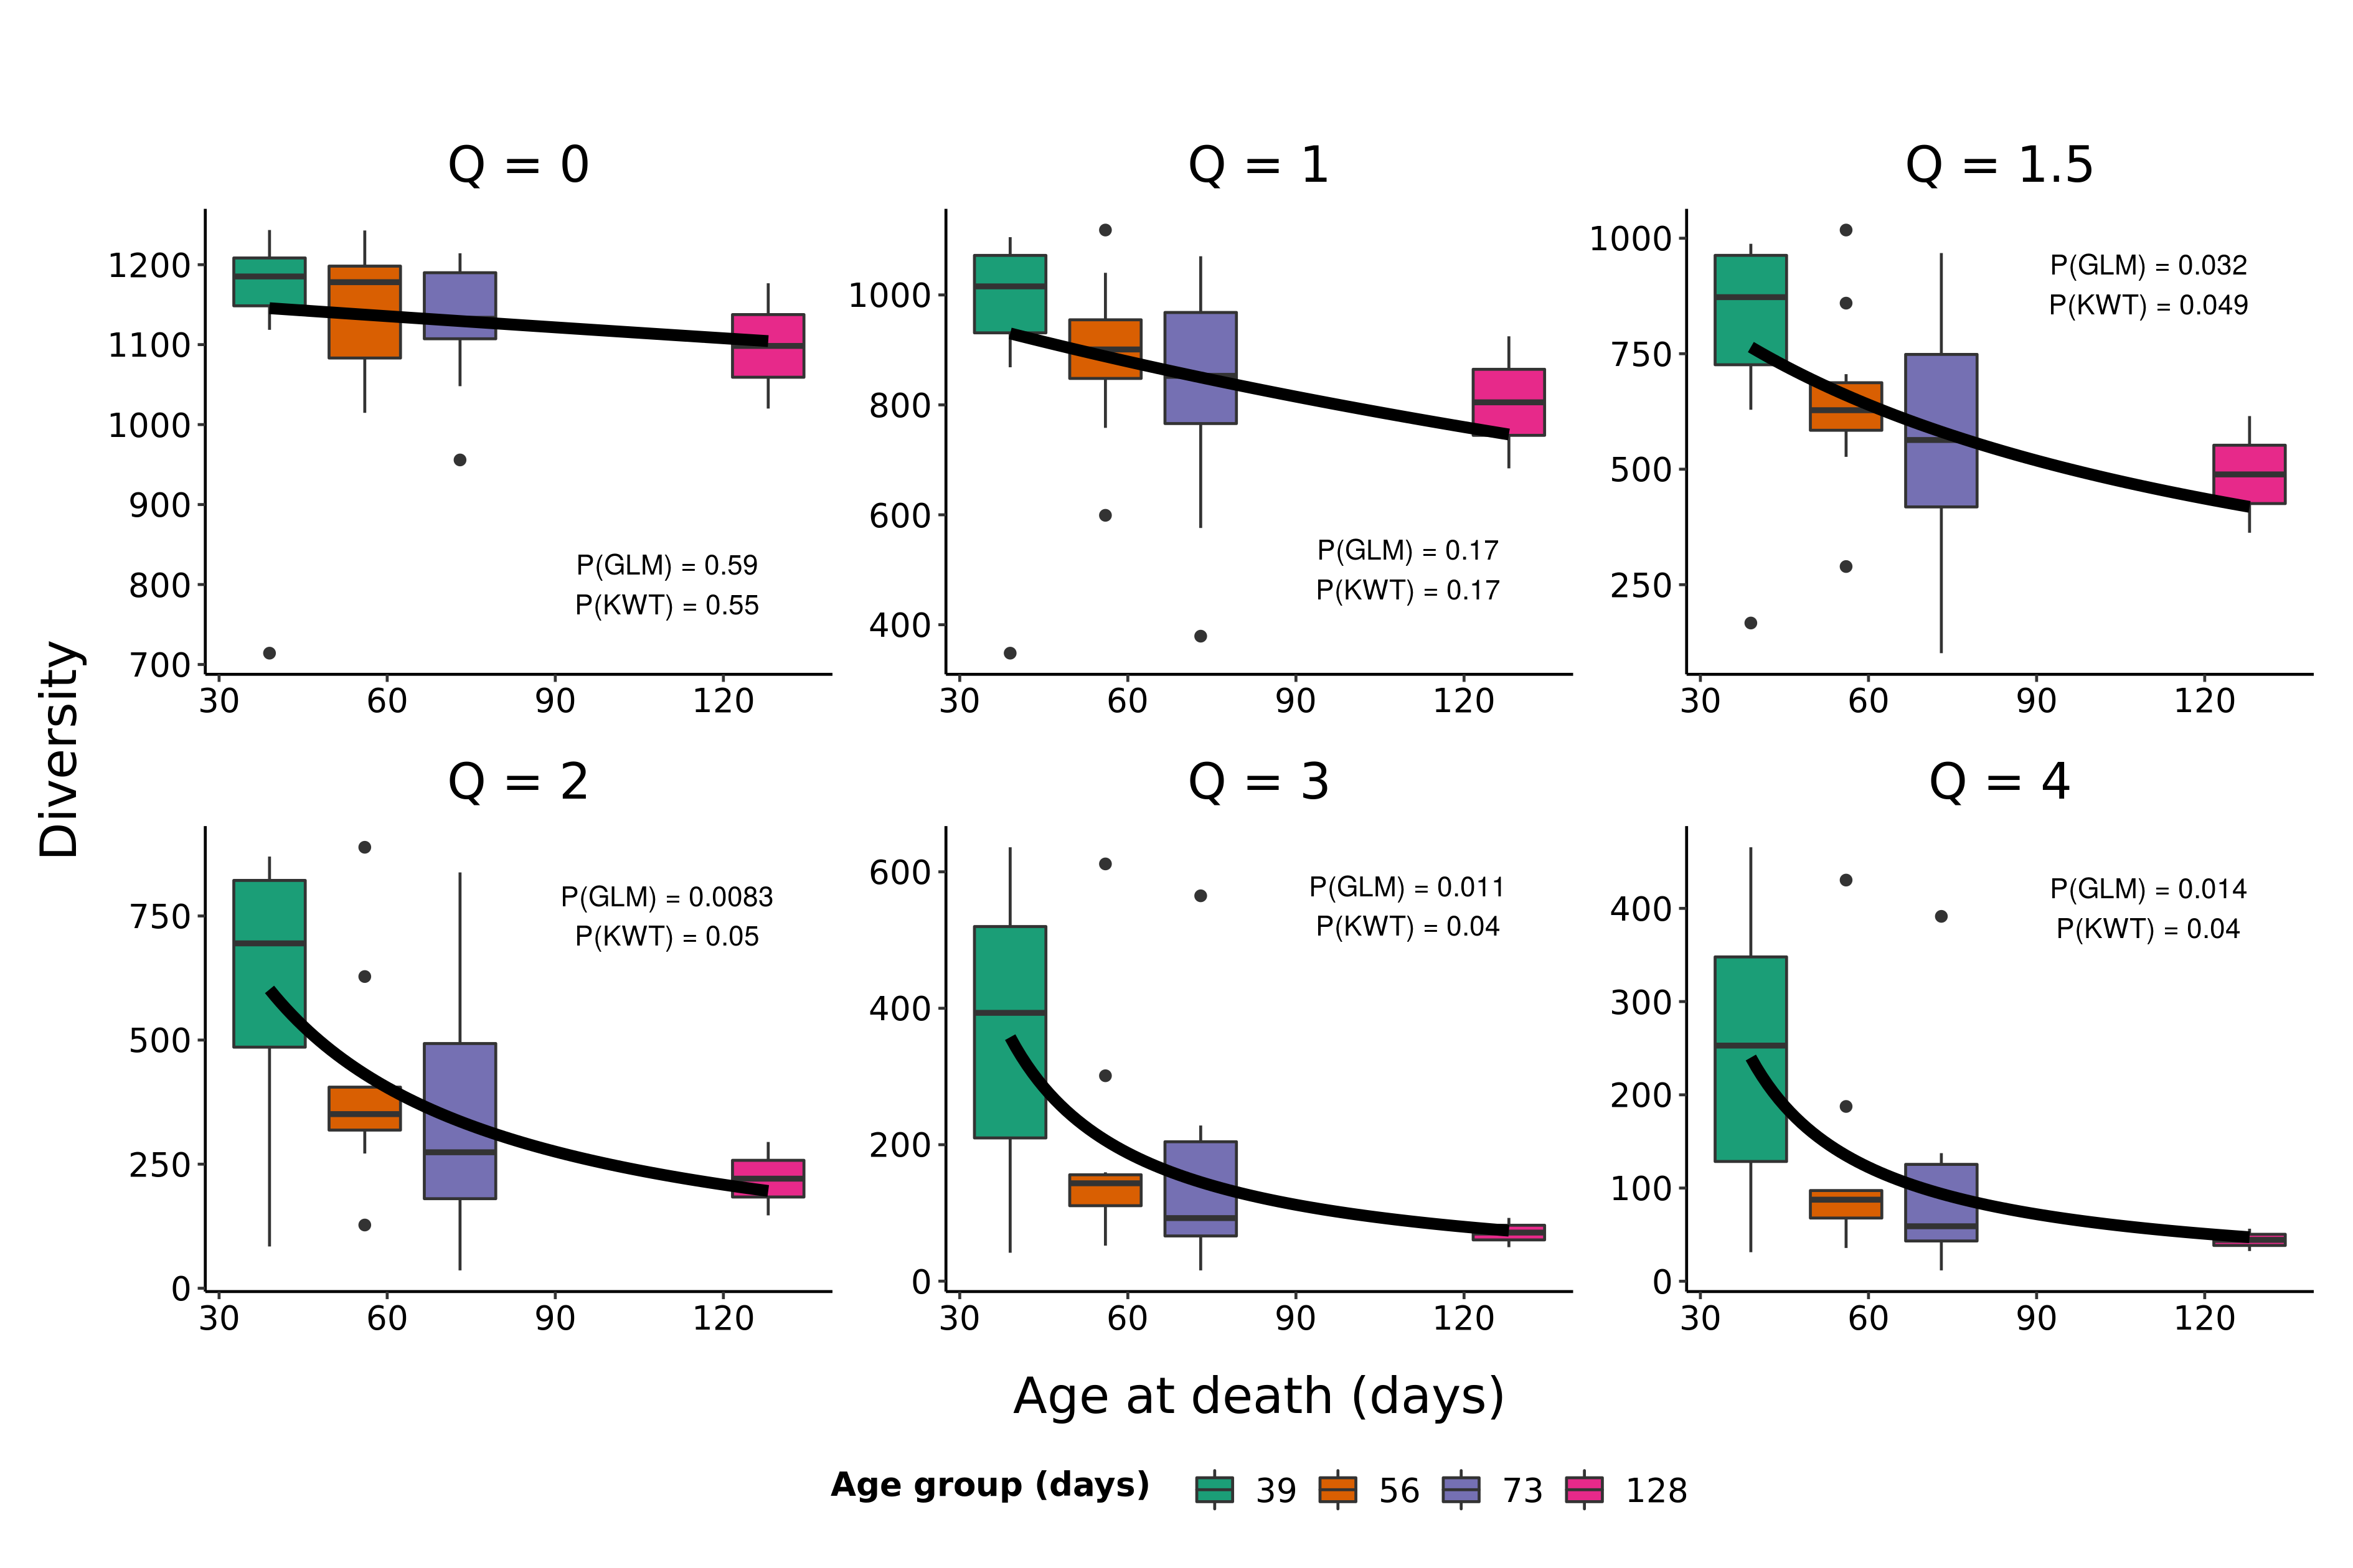
\includegraphics[width = 0.9\textwidth]{_Figures/png/ageing-clone-diversity-solo-fit-gamma}
\caption[Comparing clonal alpha-diversities between age groups in the \igseq ageing dataset]{\textbf{Comparing clonal alpha-diversities between age groups in the \igseq ageing dataset:} Boxplots of Hill diversity values for the antibody repertoires of individuals of each age group in the \igseq ageing dataset at a sample of diversity orders, overlaid with the predictions of the best-fit Gamma-distributed generalised linear model at each order.  Annotated $p$-values indicate the statistical significance of the estimated age effect on diversity under the GLM ($P(GLM)$) and a Kruskal-Wallis test ($P(KWT)$) for each diversity order.}
\label{fig:igseq-ageing-clone-diversity-solo-fit-gamma}
\end{figure}

While a significant decline in clonal diversity was age was found at various diversity orders, no such decline was observed in the VJ-repertoires of the different age-groups, either when visually comparing the alpha-spectra (\Cref{fig:igseq-ageing-VJ-diversity-alpha}) or statistically comparing the distributions at different diversity orders (\Cref{fig:igseq-ageing-VJ-diversity-solo-fit-gamma}). This marked difference between the clonal and VJ repertoires is at first surprising, as a distortion in the clonal repertoire caused by an increased dominance of a few large clones might be expected to cause a similar distortion in the VJ repertoire by expanding those dominant clones' V/J combinations; however, given that an average of \embed{_Figures/txt/ageing-pc-seq-in-small-clones-avg.txt}\,\% of unique sequences in the repertoire are contained in small clones of fewer than 5 unique sequences (\Cref{fig:igseq-ageing-pc-seq-in-small-clones}), and that this average does not change significantly with age (Kruskal-Wallis analysis of variance, $p=\embed{_Figures/txt/ageing-pc-seq-in-small-clones-kruskal-p.txt}$), it may simply be the case that any age-related change in VJ-diversity arising from the minority of sequences in expanded clones is dominated by an absence of change in the V/J-usage distribution of \naive B-cells. % TODO: To test this hypothesis...

% TODO: Test diversity of activated clones
% TODO: Test change in V/J usage entropy with age with IGoR

\begin{figure}
\centering
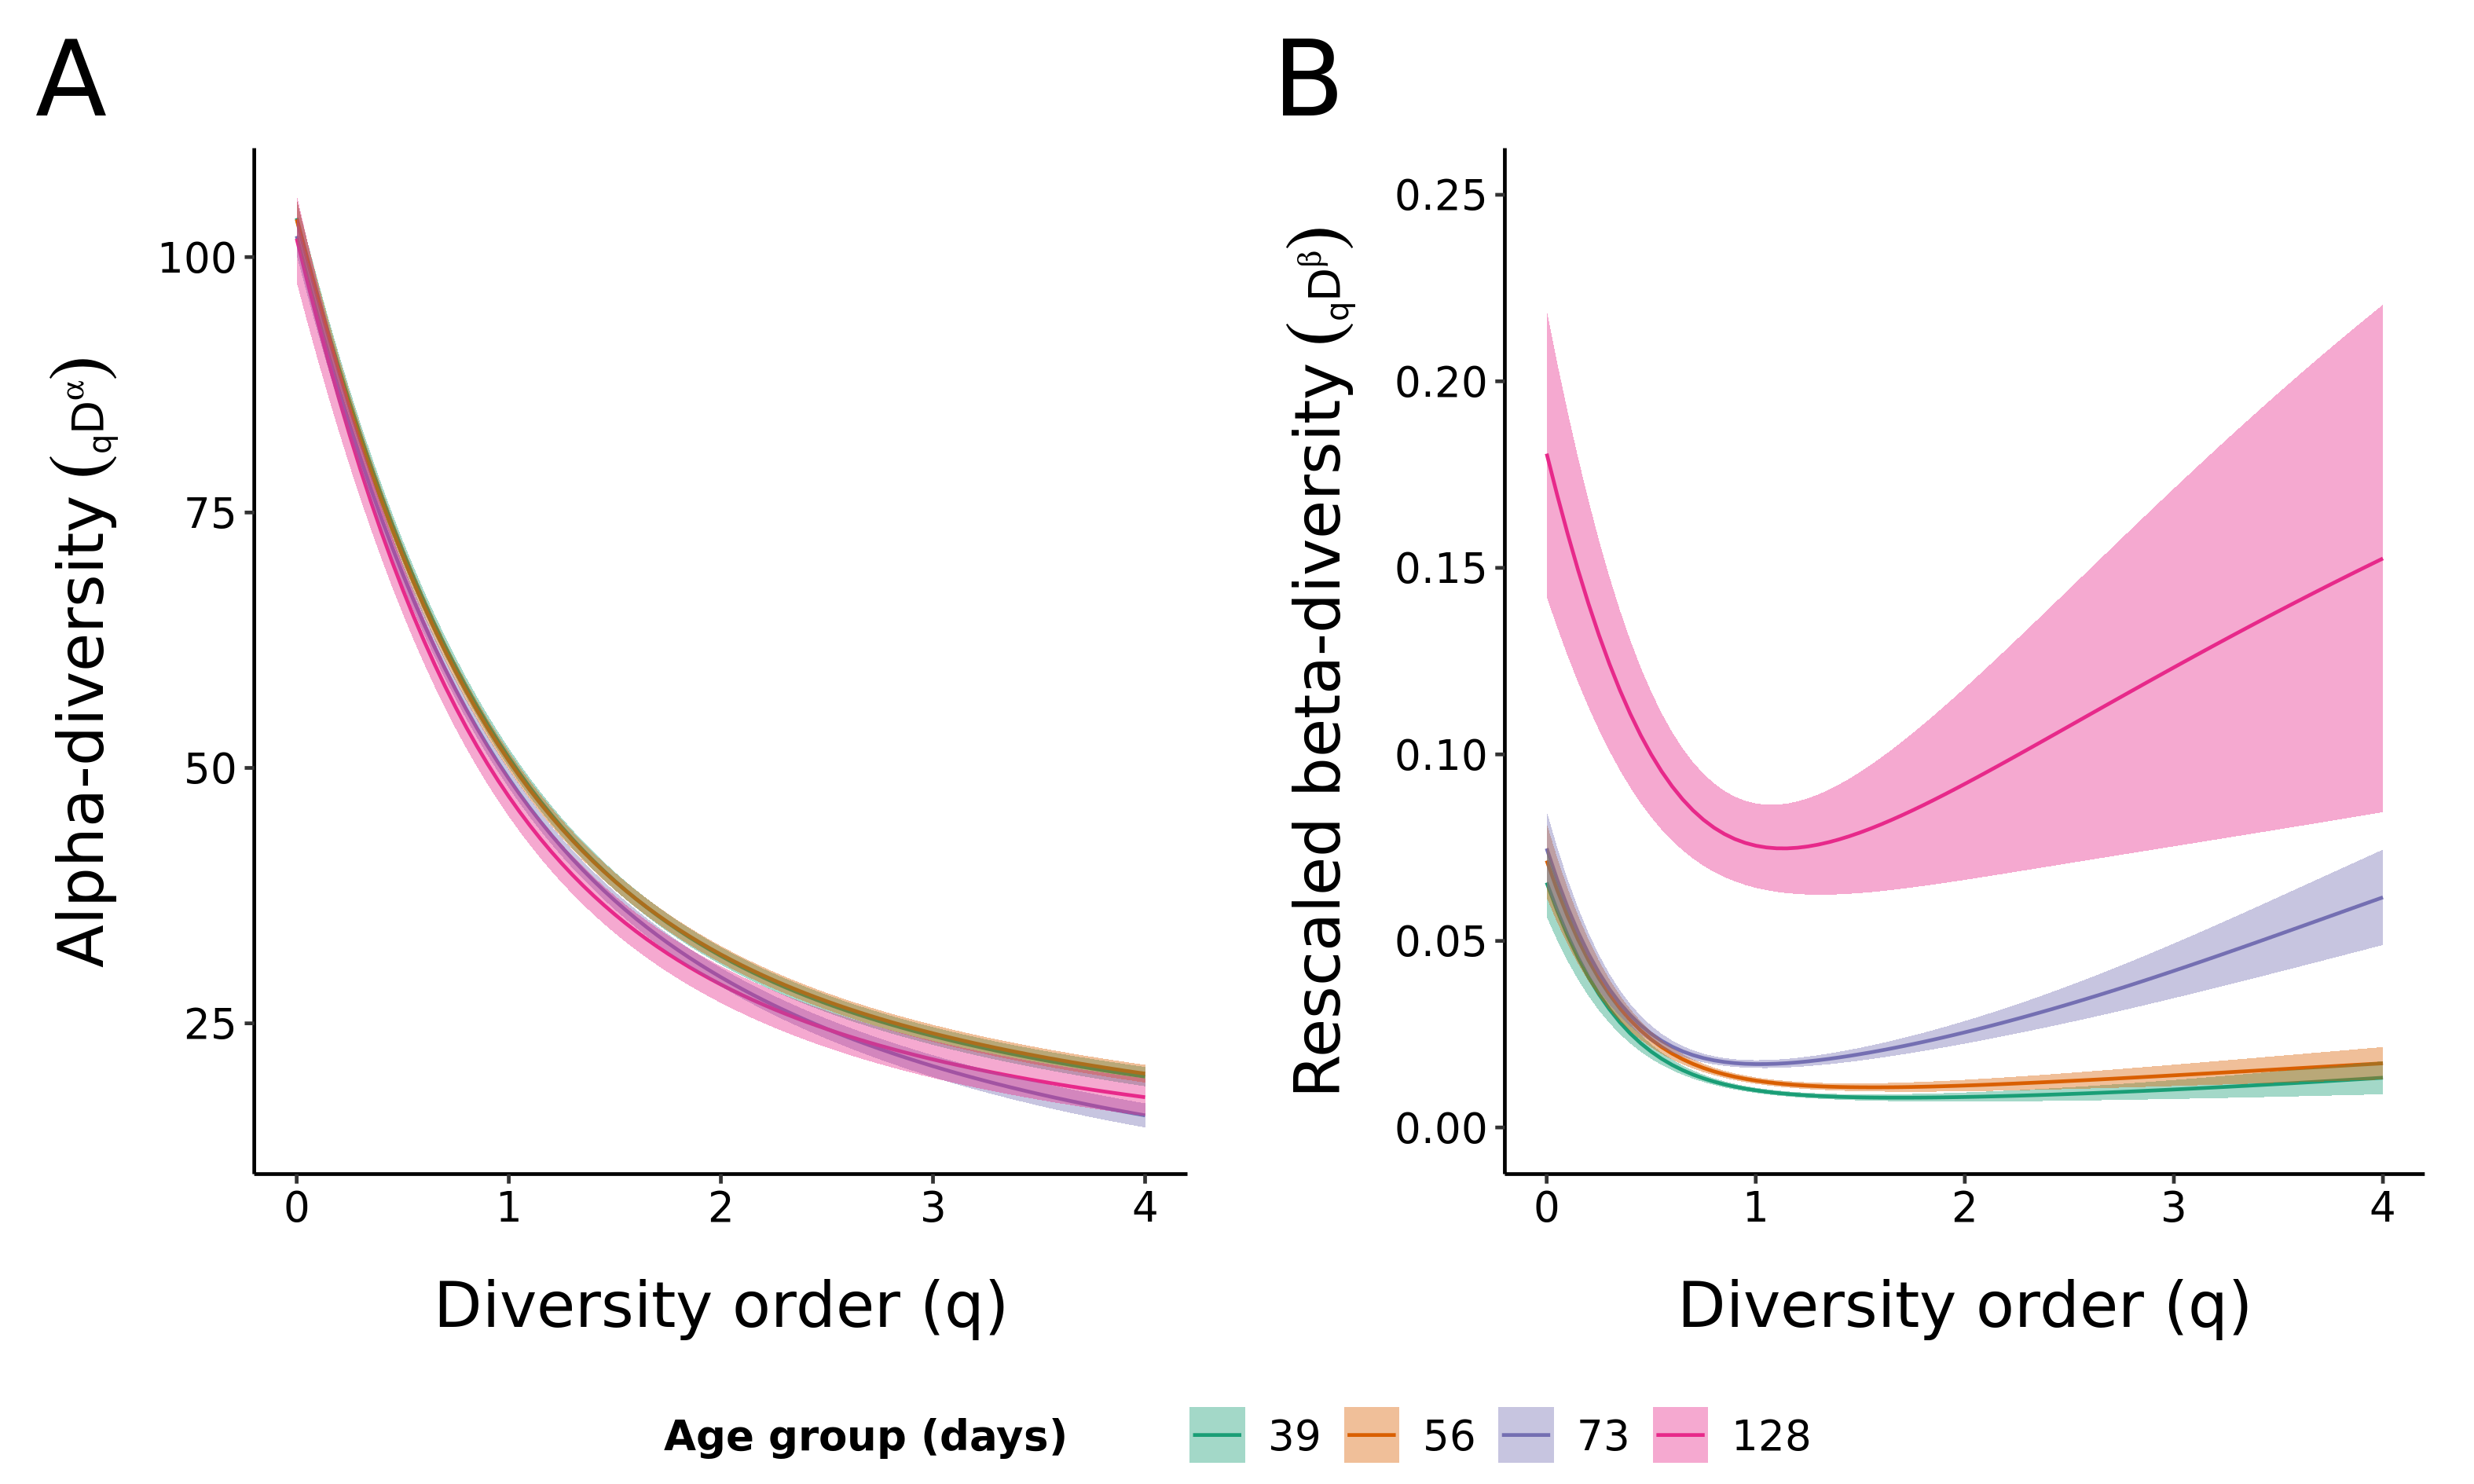
\includegraphics[width = 0.8\textwidth]{_Figures/png/ageing-VJ-diversity-alpha-beta}
\begin{subfigure}{0em}
\phantomsubcaption{}
\label{fig:igseq-ageing-VJ-diversity-alpha}
\end{subfigure}
\begin{subfigure}{0em}
\phantomsubcaption{}
\label{fig:igseq-ageing-VJ-diversity-beta}
\end{subfigure}
\caption[VJ-diversity spectra for \igseq ageing dataset]{\textbf{VJ-diversity spectra for \igseq ageing dataset:} Bootstrapped Hill diversity spectra of VJ usage (as measured by number of unique sequences per unambiguous V/J combination) over individuals for each age group in the \igseq ageing dataset. (A) Alpha-diversity across individuals; (B) Beta-diversity across individuals, rescaled to between 0 (minimum) and 1 (maximum) in accordance with the number of individuals in each age group. Shaded regions in both subfigures represent 95\,\% confidence intervals, estimated using bootstrapping.}
\label{fig:igseq-ageing-VJ-diversity-spectra}
\end{figure}

\begin{figure}
\centering
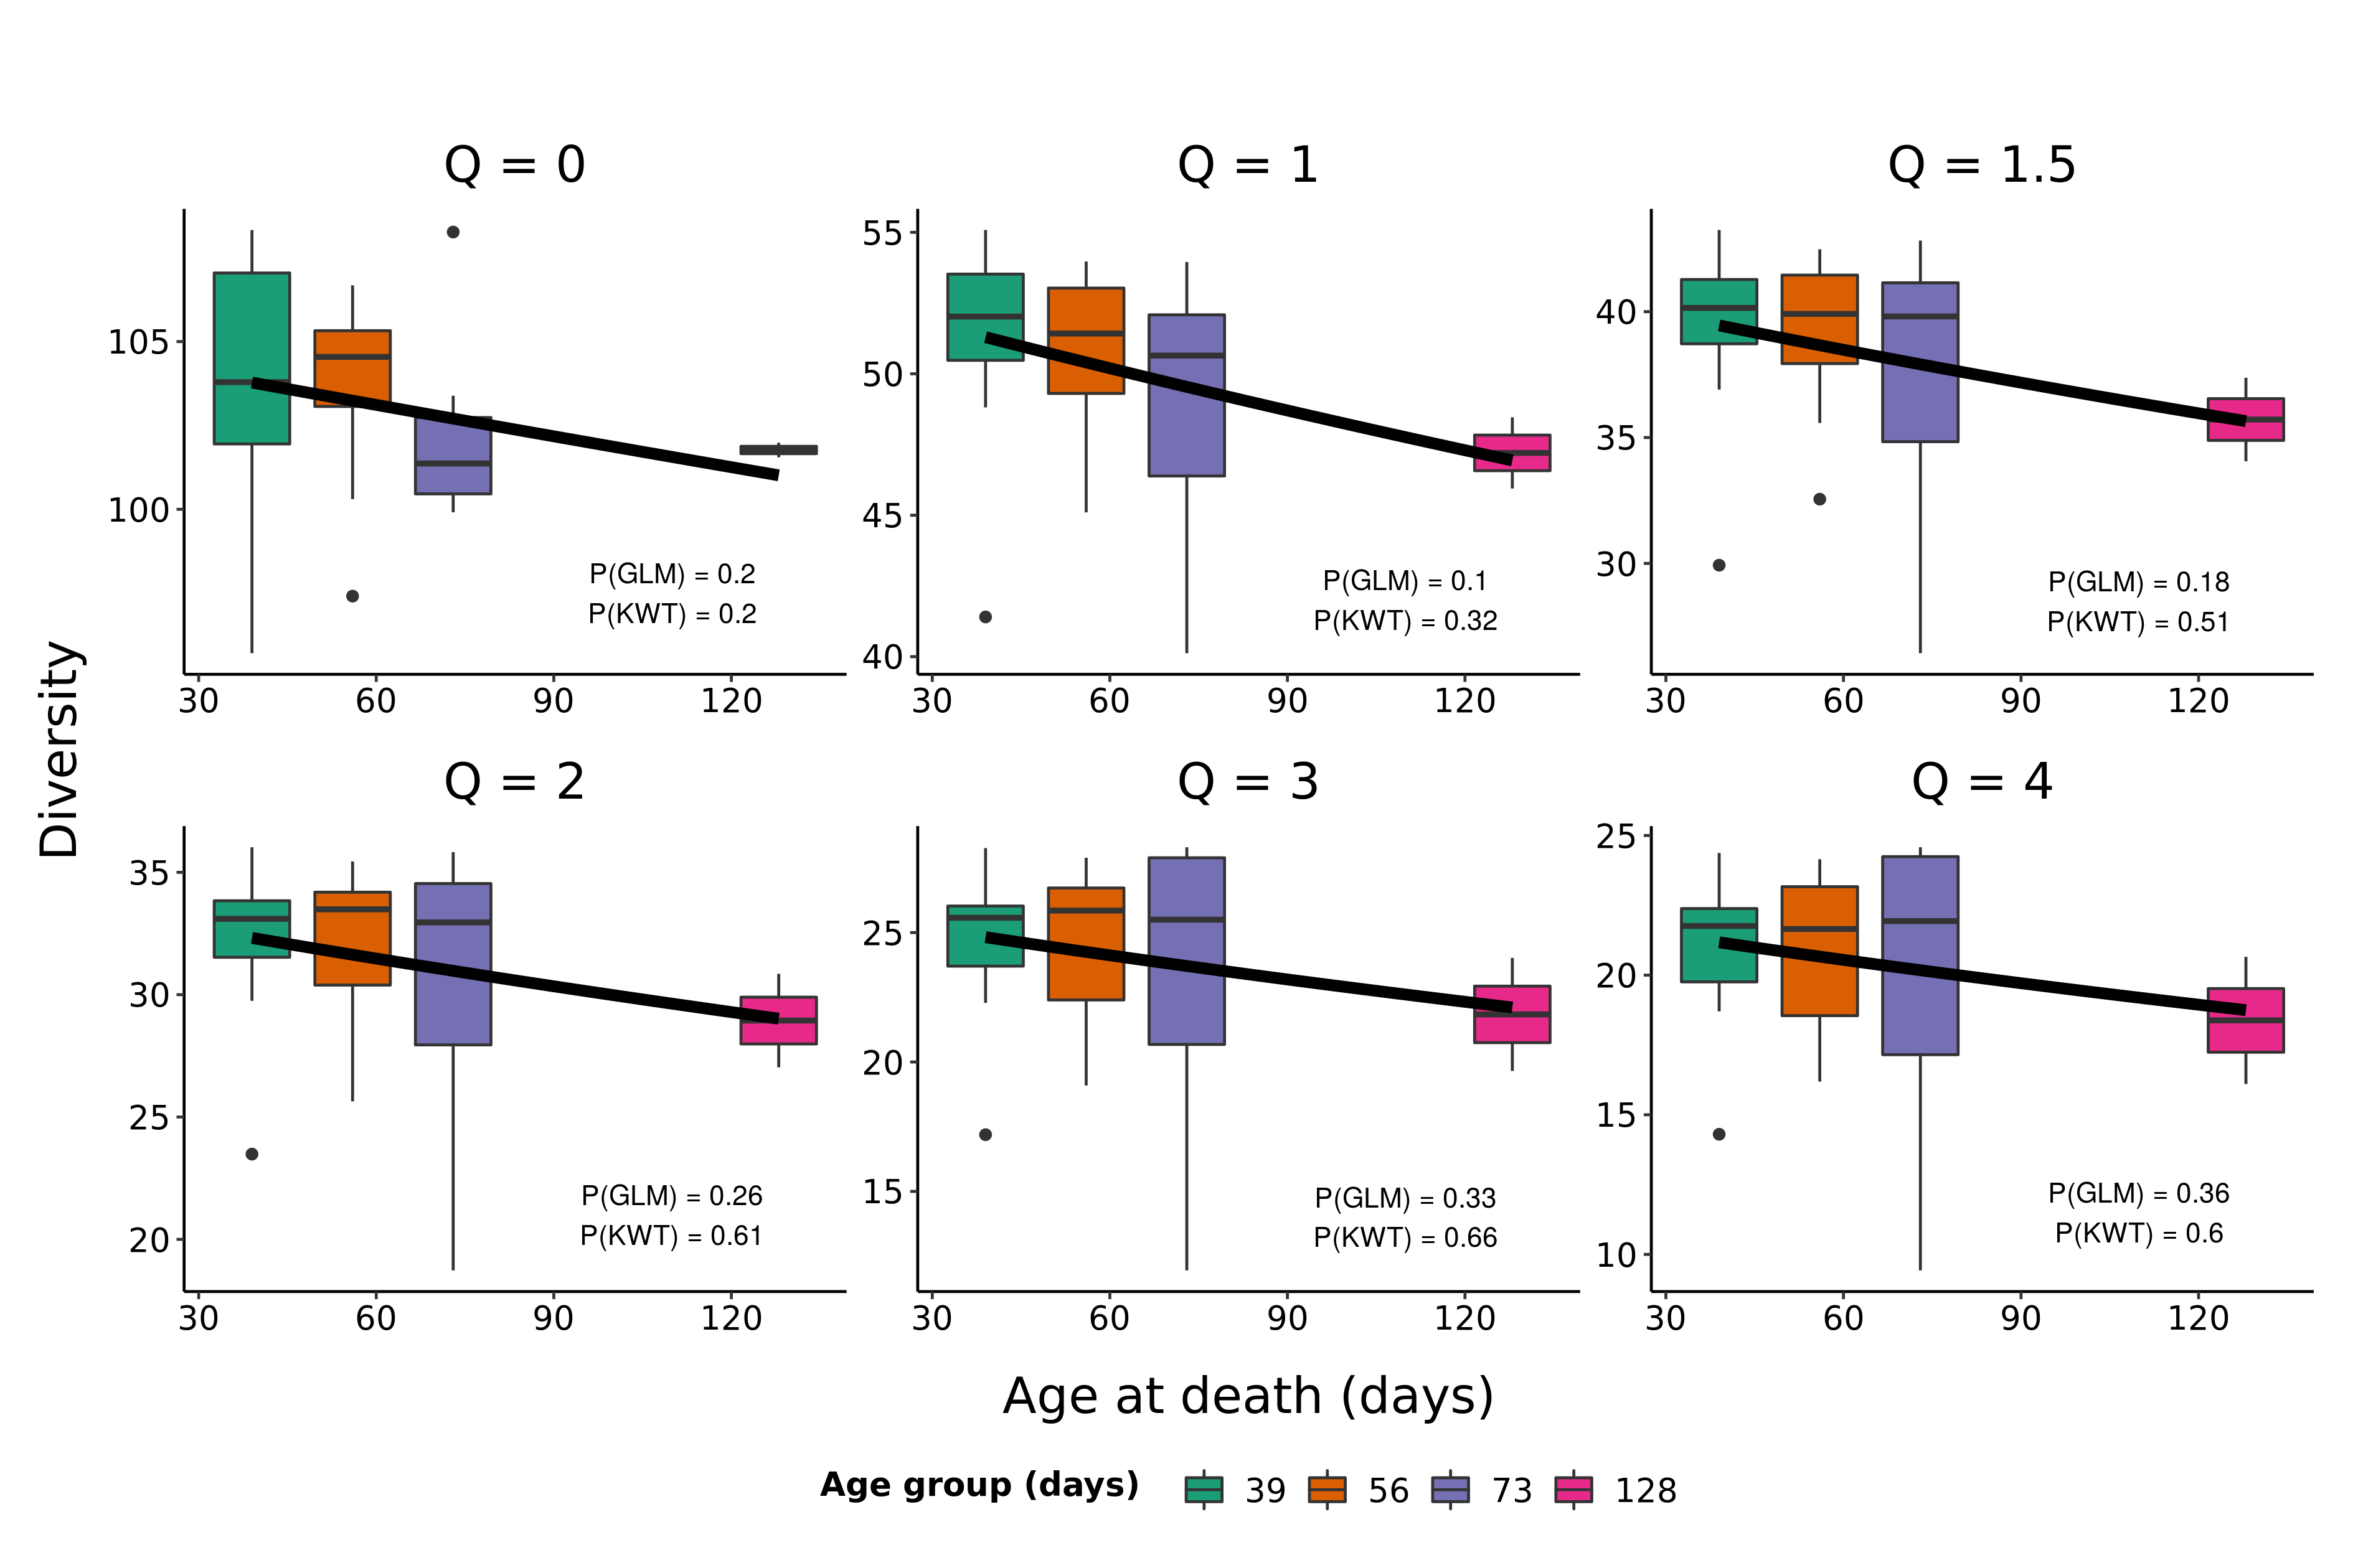
\includegraphics[width = 0.8\textwidth]{_Figures/png/ageing-VJ-diversity-solo-fit-gamma}
\caption[Comparing VJ alpha-diversities between age groups in the \igseq ageing dataset]{\textbf{Comparing VJ alpha-diversities between age groups in the \igseq ageing dataset:} Boxplots of Hill diversity values for the VJ repertoires of individuals of each age group in the \igseq ageing dataset at a sample of diversity orders, overlaid with the predictions of the best-fit Gamma-distributed generalised linear model at each order.  Annotated $p$-values indicate the statistical significance of the estimated age effect on diversity under the GLM ($P(GLM)$) and a Kruskal-Wallis test ($P(KWT)$) for each diversity order.}
\label{fig:igseq-ageing-VJ-diversity-solo-fit-gamma}
\end{figure}

While the alpha-diversity of the VJ-repertoire (reflecting average diversity within each individual repertoire) does not appear to change with age in the turquoise killifish, the beta-diversity (reflecting inter-individual variability in VJ-expression) shows dramatic differences between age groups, especially at higher diversity orders (\Cref{fig:igseq-ageing-VJ-diversity-beta}): while the diversity of the 5.5- and 8-week-old groups is close to the theoretical minimum for that sample size, the 10.5-week-old group exhibits a substantial increase in inter-individual variability across a wide range of diversity orders, and the 18-week old group shows an even more dramatic increase. This increase in inter-individual diversity with age is corroborated by inter-individual RDI distances computed on VJ-repertoires within each age group: both the overall distribution of inter-individual distances (\Cref{fig:igseq-ageing-rdi-VJ-individual-groupdist-all}), and the distribution of nearest-neighbour distances within each age group (\Cref{fig:igseq-ageing-rdi-VJ-individual-groupdist-nn}), increase significantly with age. This tendency for individuals from increasing age groups to become more distinct in their VJ-repertoires can also be observed using principal co-ordinate analysis:  in \Cref{fig:igseq-ageing-rdi-VJ-individual-pcoa-facet}, the great majority of individuals from younger age groups are visibly more tightly clustered than those from older age groups, which drift apart progressively as age-at-death increases. As in ageing humans (\Cref{sec:intro_immunosenescence}), therefore, the ageing killifish appears to become more individualised and distinct in its antibody repertoire, presumably as the result of an accumulating history of unique individual responses to antigen exposure.

\begin{figure}
\centering
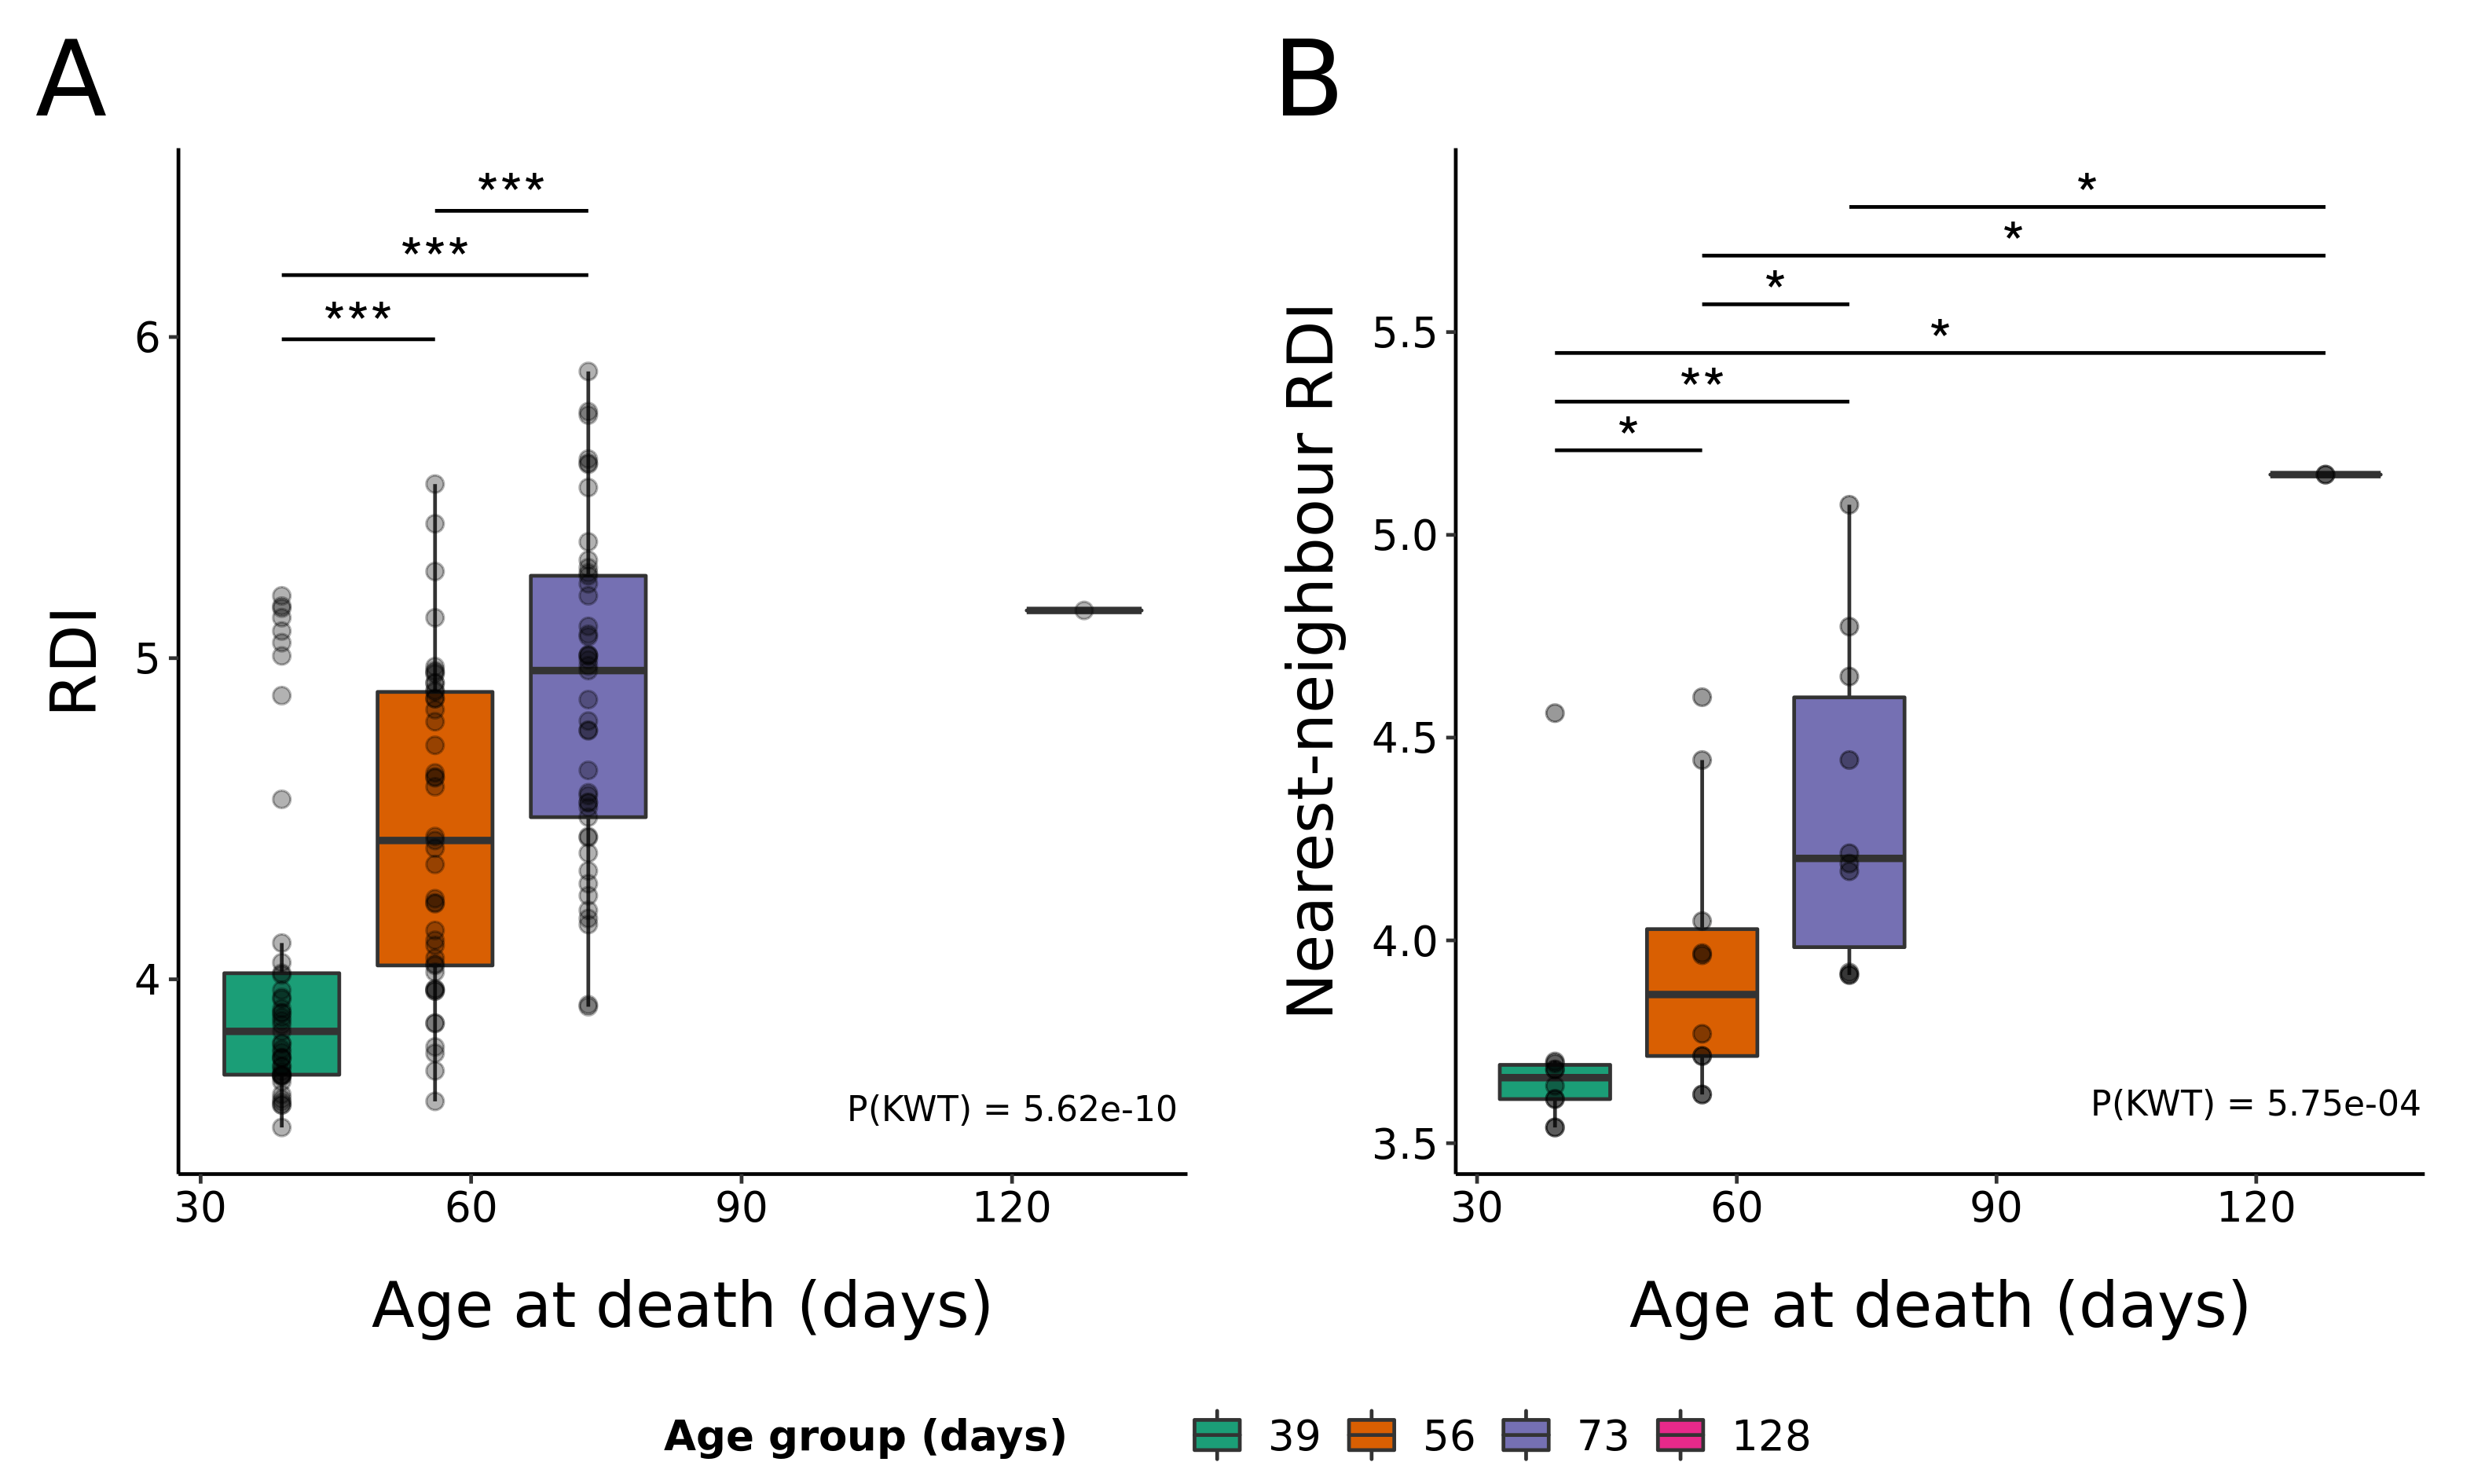
\includegraphics[width = 0.9\textwidth]{_Figures/png/ageing-rdi-VJ-individual-groupdist}
\begin{subfigure}{0em}
\phantomsubcaption{}
\label{fig:igseq-ageing-rdi-VJ-individual-groupdist-all}
\end{subfigure}
\begin{subfigure}{0em}
\phantomsubcaption{}
\label{fig:igseq-ageing-rdi-VJ-individual-groupdist-nn}
\end{subfigure}
\caption[Inter-individual VJ-RDI distances in the \igseq ageing dataset, part 1]{\textbf{Inter-individual VJ-RDI distances in the \igseq ageing dataset, part 1:} Boxplots of overall (A) and nearest-neighbour (B) inter-individual VJ-RDI distances for each age group in the \igseq ageing dataset. Pairwise $p$-values are computed using nonparametric Mann–Whitney U tests ($*: 0.01 < p \leq 0.05;~**: 0.001 < p \leq 0.01;~***: p \leq 0.001$). $P(KWT)$ indicates the $p$-value of a Kruskal-Wallis analysis of variance test for a difference in RDI distribution with age.}
\label{fig:igseq-ageing-rdi-VJ-individual-groupdist}
\end{figure}

\begin{figure}
\centering
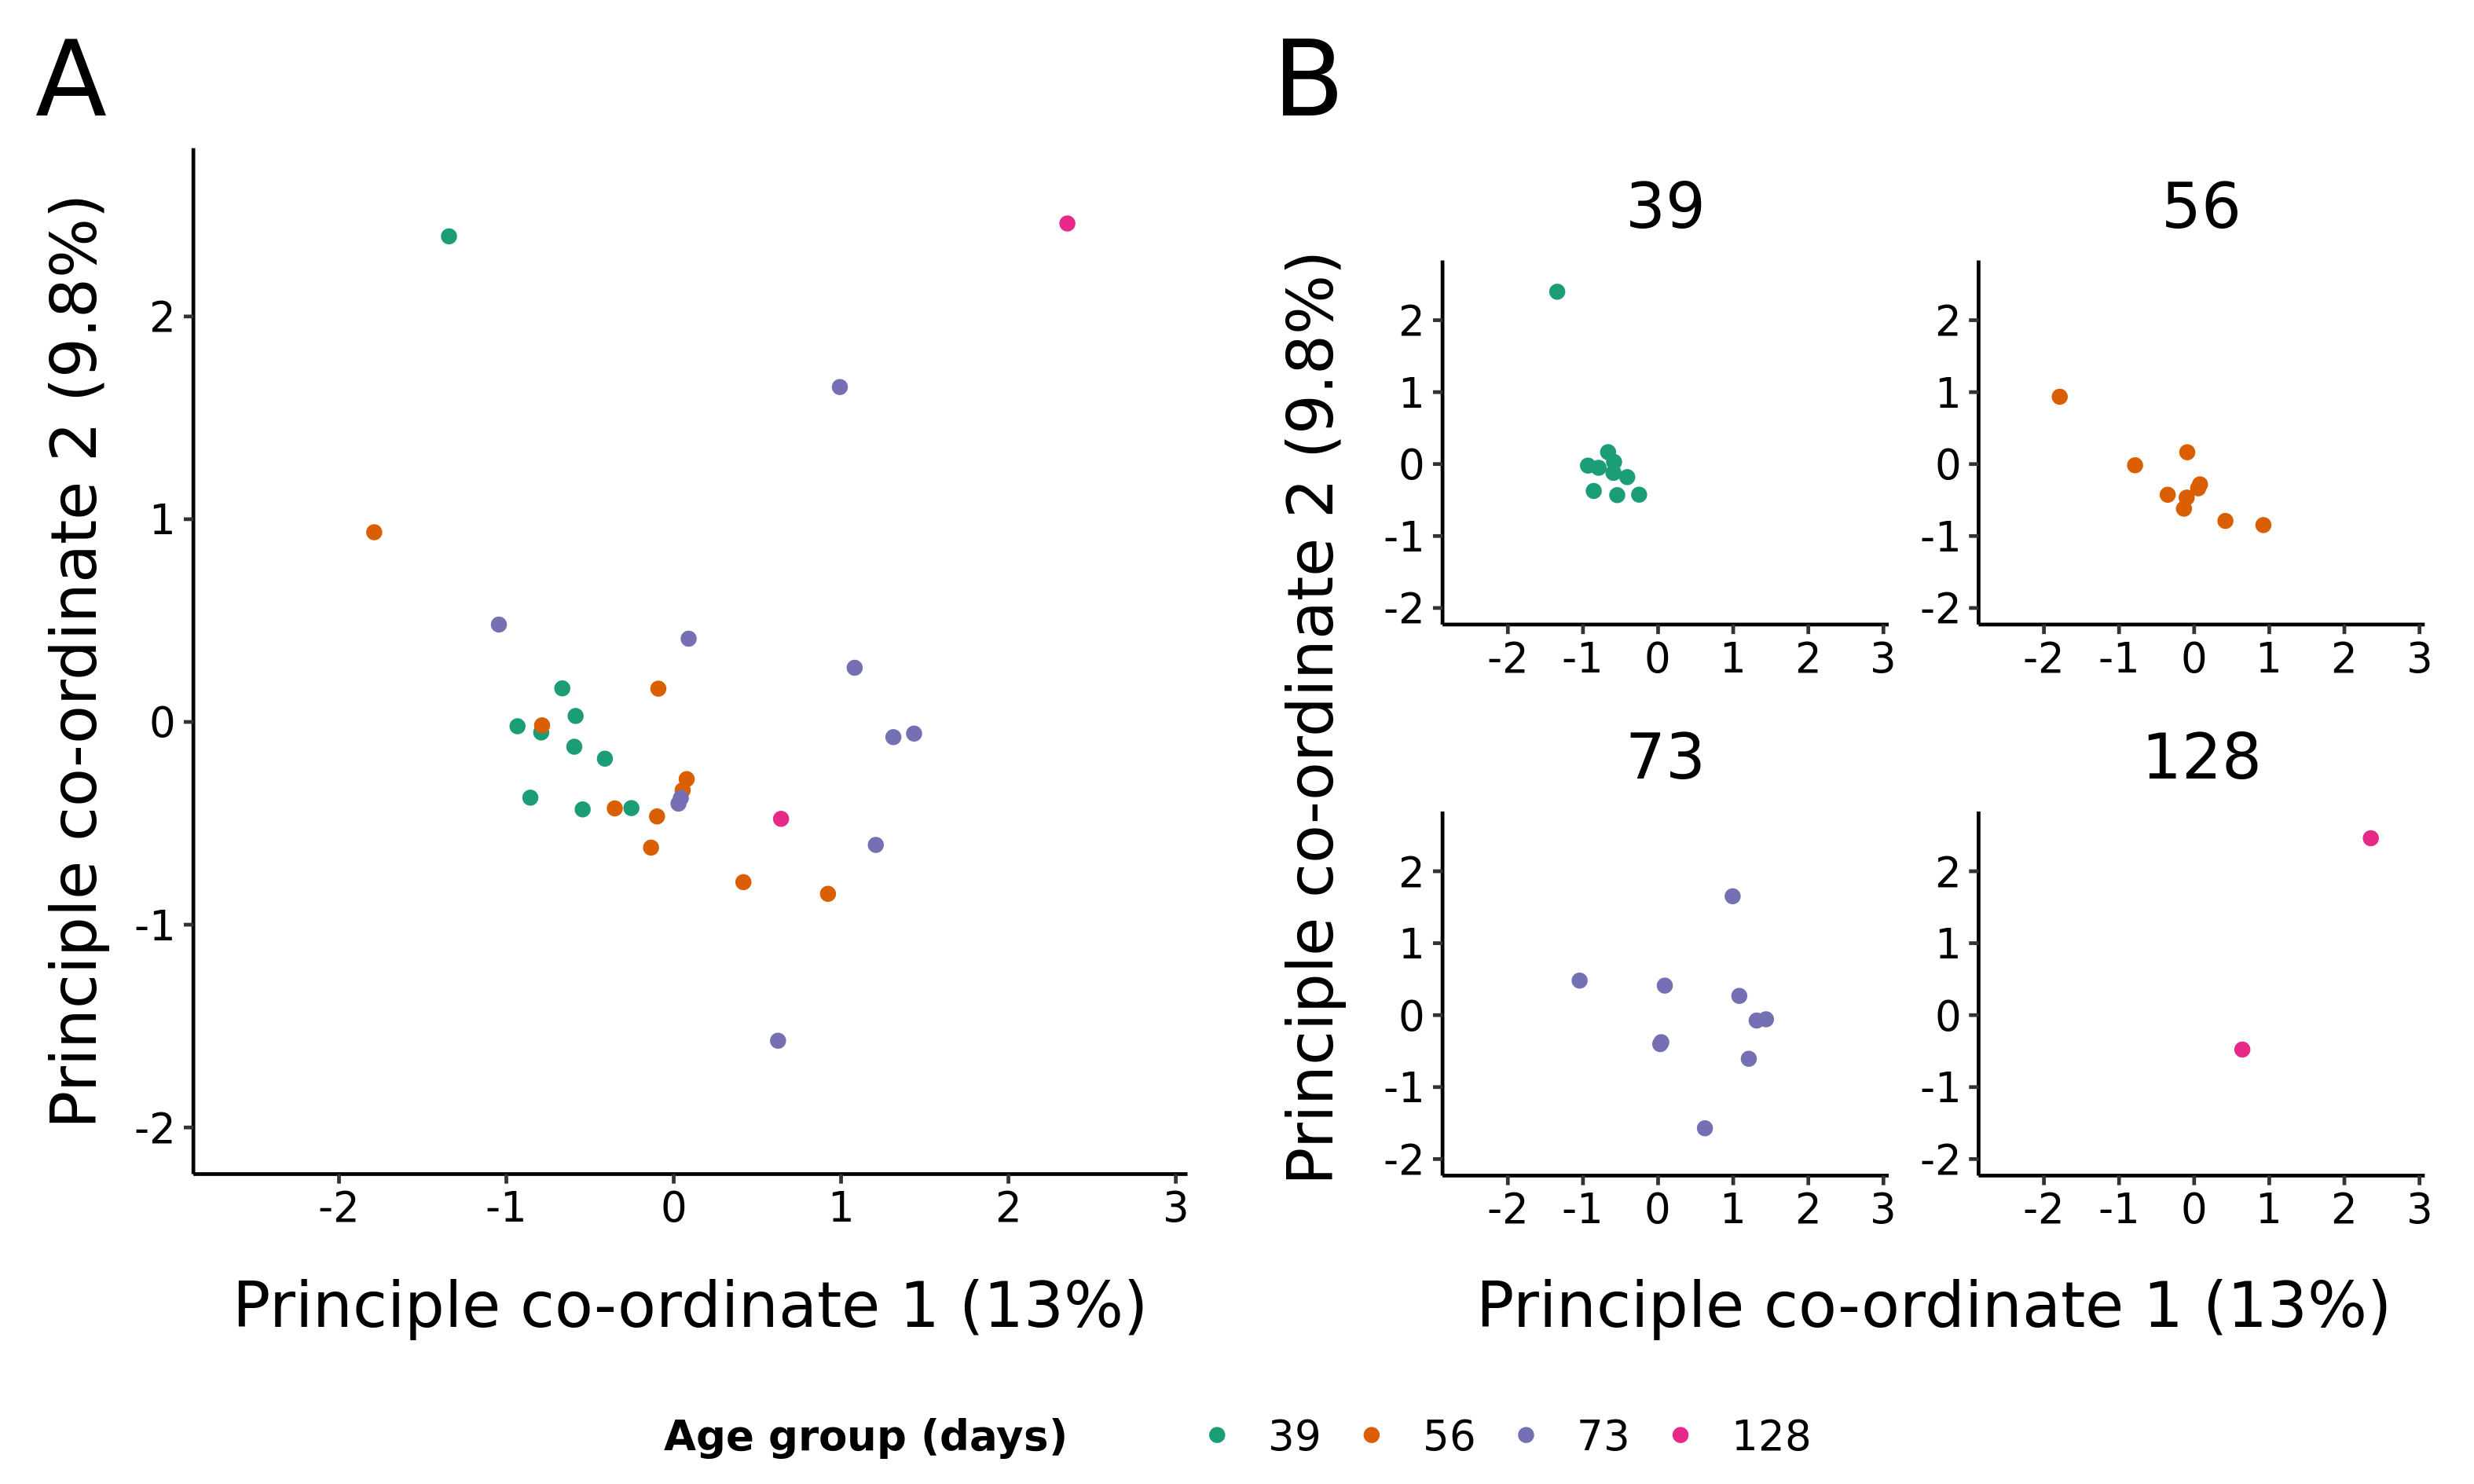
\includegraphics[width = 0.9\textwidth]{_Figures/png/ageing-rdi-VJ-individual-pcoa}
\begin{subfigure}{0em}
\phantomsubcaption{}
\label{fig:igseq-ageing-rdi-VJ-individual-pcoa-all}
\end{subfigure}
\begin{subfigure}{0em}
\phantomsubcaption{}
\label{fig:igseq-ageing-rdi-VJ-individual-pcoa-facet}
\end{subfigure}
\caption[Inter-individual VJ-RDI distances in the \igseq ageing dataset, part 2]{\textbf{Inter-individual VJ-RDI distances in the \igseq ageing dataset, part 2:}Principal co-ordinate analysis (PCoA) of pairwise inter-individual VJ-RDI distances in the \igseq ageing dataset, coloured by age group and displayed together (A) or separately by age group (B).}
\label{fig:igseq-ageing-rdi-VJ-individual-pcoa}
\end{figure}

% TODO: Simple measures of selection: CDR3 length, # STOP codons

% TODO: IGoR parameters and entropy with age

% TODO: Conclusion: effects of ageing on repertoire composition in TK

\FloatBarrier
\clearpage